%% \documentclass[draft]{beamer}
\documentclass[serif]{beamer}
\usepackage{graphicx}
\usepackage{amsfonts}
\usepackage{amsmath}
\usepackage{algorithm2e}
\usepackage{rotating}
\usepackage{/home/sci/weiliu/haldefs}

\usetheme{Warsaw}
\setbeamertemplate{navigation symbols}{}
\renewcommand\mathfamilydefault{\rmdefault}

\renewcommand{\inserttotalframenumber}{30}
\setbeamertemplate{footline}[page number] % add page number

\title[Functional Connectivity by Multi-Level MRF]{Functional Connectivity of Resting-State fMRI }
\subtitle{A Group Study By Multi-Level Markov Random Field}
\author[W. Liu]{Wei Liu}
\institute[SCI]{
  Scientific Computing and Imaging Institute\\
  University of Utah
}
\date{\today}
\begin{document}

\begin{frame}
  \titlepage
\end{frame}

\begin{frame}
  \frametitle{Why Resting-State fMRI}

  \hfill 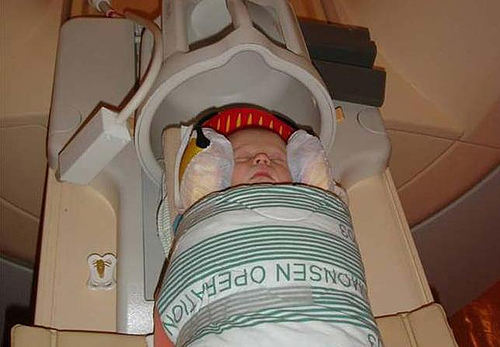
\includegraphics[width=0.2\textwidth]{sfig/baby}
  \vspace{10pt}
    \begin{block}{Intrinsic v.s. Reflective}
      Interpret, respond to, and predict environmental demands.
  \end{block}

  \begin{block}{Why Resting-State}
    \begin{itemize}
      \item Large energy consumption.
        \item Matches existing neuro-anatomical systems.
          \item Reflect increased and decreased activity in task.
            \item Predict task response as a priori hypothesis.
    \end{itemize}
    \end{block}
\end{frame}
%---------------------------------------------------
\begin{frame}
  \frametitle{fMRI Data Acquisition}
  \begin{columns}[c]
    \begin{column}{4cm}
        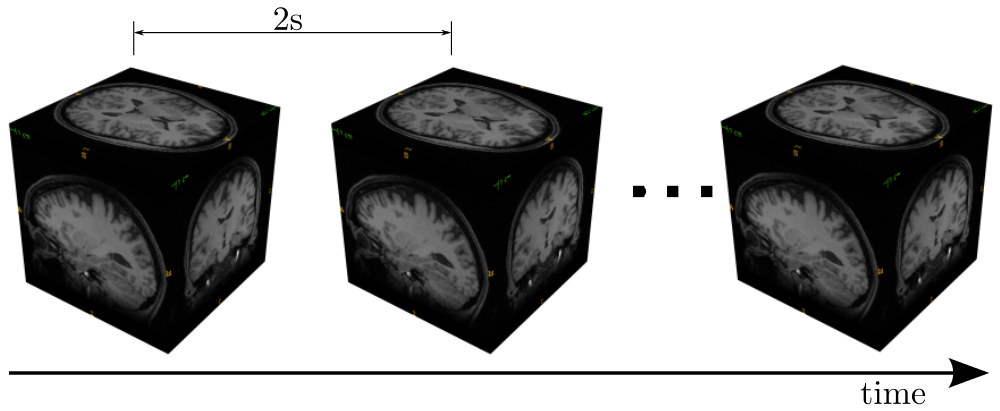
\includegraphics[width=1\textwidth]{sfig/4dfmri}
        \vspace{1cm}
        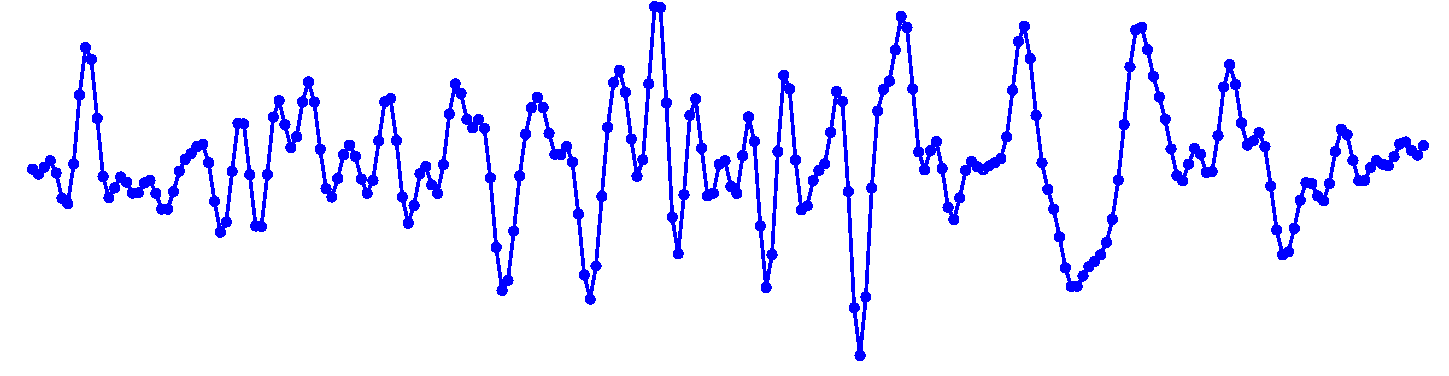
\includegraphics[width=1\textwidth]{sfig/onets}
        \vspace{1cm}
        \centering
        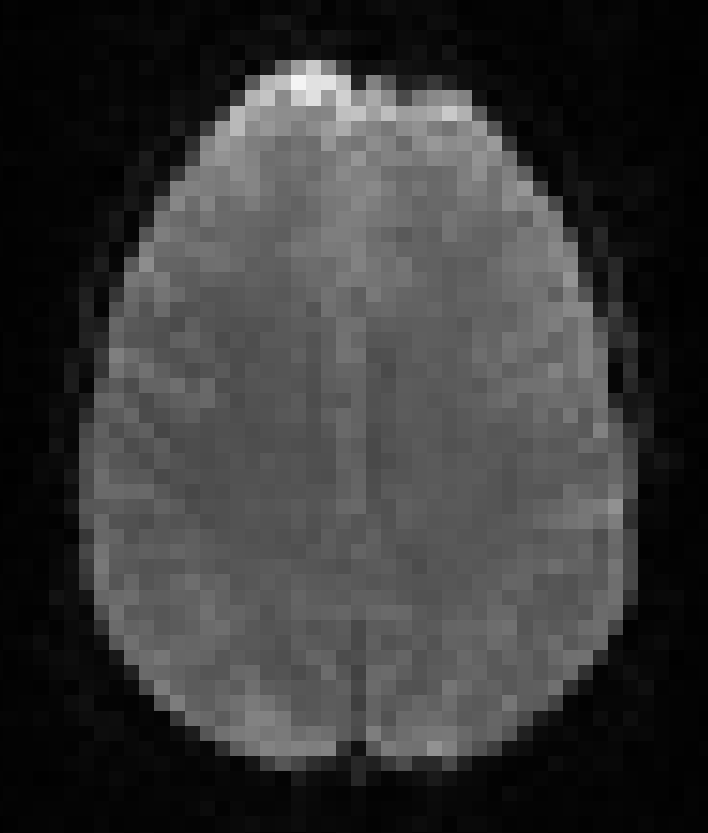
\includegraphics[width=2cm]{sfig/rawslice}
    \end{column}

    \begin{column}{6cm}
      \begin{block}{}
        \begin{itemize}
        \item fMRI is 4D. Many consecutive 3D volumes.
        \item BOLD signal.
        \item Spatial dependency.
        \item Temporal correlation.
        \item fMRI is noisy.
        \end{itemize}
      \end{block}
    \end{column}
  \end{columns}

\end{frame}
%--------------------------------------------------------

\begin{frame}
  \frametitle{Task-based v.s. Resting-State fMRI}
  \begin{columns}[t]
    \begin{column}{5cm}
      \begin{block}{}
        \begin{itemize}
        \item Experiment stimulus signal.
        \item Subjects undertake cognitive tasks.
        \item General linear model is used for multi-regression analysis between
          stimulus and BOLD signal of a voxel.
        \end{itemize}
      \end{block}
      \begin{figure}
        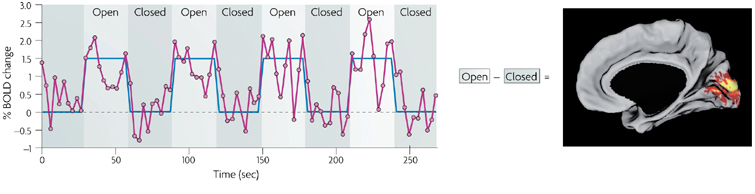
\includegraphics[width=5cm]{sfig/taskfmri}
        \caption{\tiny M. Fox, Nat. Rev., Neuroscience}
        \end{figure}

    \end{column}

    \begin{column}{5cm}
      \begin{block}{}
        \begin{itemize}
        \item No experiment paradigm signal.
        \item Subject stay in scanner. Eyes closed/open to a fixation cross.
        \item Correlation analysis between two voxels.
        \end{itemize}
      \end{block}
      \begin{figure}
        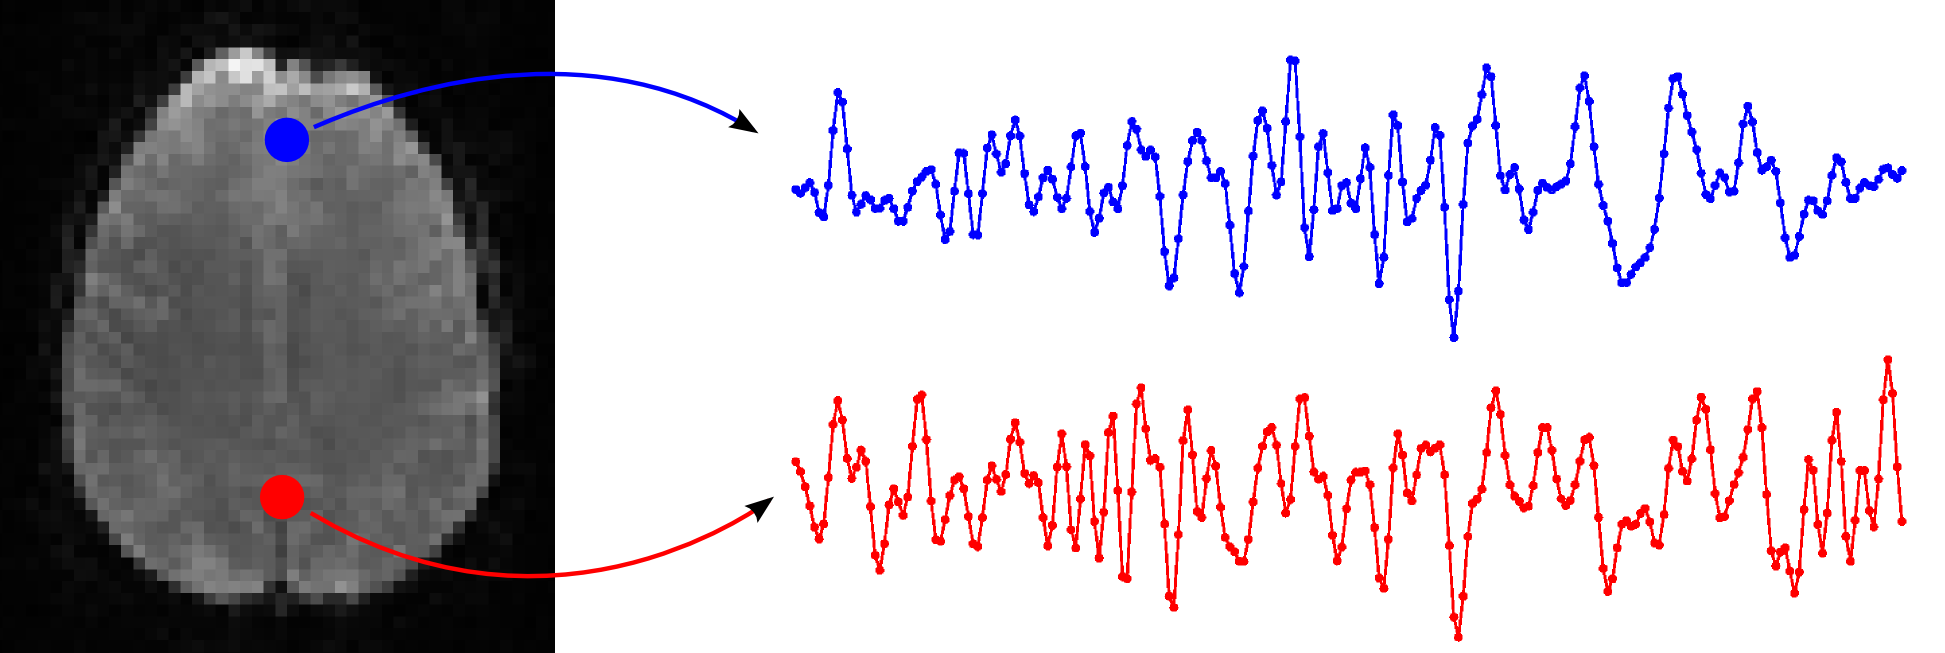
\includegraphics[width=5cm]{sfig/corr}
        \end{figure}
    \end{column}

  \end{columns}
\end{frame}

%% Unaveraged blood oxygen level dependent (BOLD) time course (magenta) from a
%% region in the primary visual cortex during a simple task paradigm that
%% requires subjects to open and close their eyes. The paradigm is shown in blue
%% (delayed to account for the haemodynamic response). Traditional functional
%% magnetic resonance imaging (fMRI) analysis involves correlating BOLD data
%% with a stimulation time-course across multiple blocks. This in effect
%% averages across each condition and performs a subtraction, minimizing 'noise'
%% in the BOLD signal and highlighting regions that are modulated by the task
%% paradigm. In this case, subtraction of the eyes-closed condition from the
%% eyes-open condition identifies a BOLD signal intensity difference in the
%% primary visual cortex (shown on the right).

\begin{frame}
\frametitle{Issues In Current Group Study}
\begin{columns}[t]
  \begin{column}{7cm}
    \begin{block}{}
      \begin{itemize}
      \item Arbitrary spatial blurring to enforce spatial dependency.
      \item Lack of methods for jointly estimate group and subjects.
      \item Variability analysis.
      \end{itemize}
      
    \end{block}
  \end{column}

  \begin{column}{3cm}
  \end{column}

\end{columns}
\end{frame}
%-----------------------------------------------------------

\begin{frame}
\frametitle{Thesis Statement} 
\begin{block}{}
  \emph{A multilevel Markov Random Field model improves the reliability of the
  functional network estimation in rs-fMRI group study by taking into account
  context information as a prior. The data-driven Bayesian model can jointly
  estimate both population and subjects' connectivity networks, as well as
  drawing inference on the uncertainty in the estimation, and on the variability
  across subjects. }
  \end{block}
\end{frame}
%---------------------------------------------
\begin{frame}
  \frametitle{Contributions}
  \begin{block}{Thesis Proposal Contributions}
    \begin{itemize}
    \item Full pairwise connectivity with spatial coherence.
    \item Identify consistent, spatially coherent multiple functional networks.
    \item Hierarchical model for group study. Estimate group and subjects together.
    \item Uncertainty and variability of resting-state functional network.
    \end{itemize}
  \end{block}
\end{frame}
%----------------------------------------------
\begin{frame}
\frametitle{Markov Random Field}
\begin{columns}
  \begin{column}{3cm}
    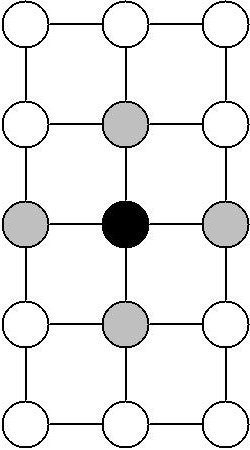
\includegraphics[width=3cm]{sfig/mrf}
  \end{column}

  \begin{column}{7cm}
    \begin{definition}
      $\mathcal{G} = (\mathcal{V}, \mathcal{E})$: undirected graph.\\
      $s \in \mathcal{V}$: a node/site in $\mathcal{V}$. \\
      $X = \{x_1, \dots, x_s, \dots \}$: a collection of random variables defined on graph $\mathcal{G}$.\\
      $\mathcal{N}_s$: the set of sites neighboring $s$. $(r,s) \in \mathcal{E} \Leftrightarrow  r\in \mathcal{N}_s $.
    \end{definition}

    \begin{definition}
      A \alert{Markov Random Field} is a collection of variables $X$ defined on
      graph $\mathcal{G} = (\mathcal{V}, \mathcal{E})$ if for all $s \in
      \mathcal{V}$
      \begin{equation*}
        P(X_s | X_{\mathcal{V}-s}) = P(X_s | X_{\mathcal{N}_s})
      \end{equation*}
    \end{definition}
  \end{column}
  \end{columns}
\end{frame}

\begin{frame}
\frametitle{Markov Random Field Cont.}
\hfill       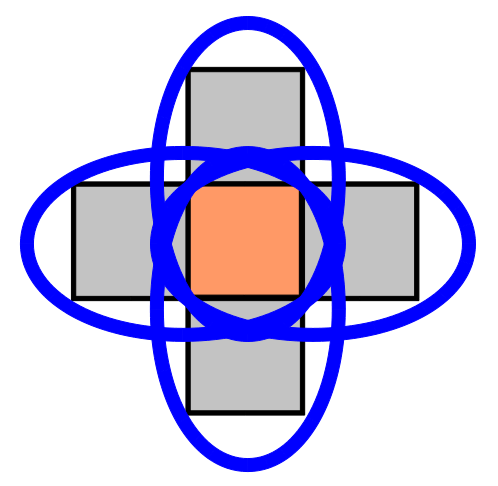
\includegraphics[width=0.15\textwidth]{sfig/clique_1}

The definition of MRF is a local property. 
\begin{theorem}[Hammersley-Clifford, 1971]
  $X$ is an MRF on $\mathcal{G}$ if and only if $X$ obeys Gibbs distribution in
  the following form
  \begin{equation*}
    P(X) = \frac{1}{Z}\exp \left( -\frac{1}{T} U(X) \right),
  \end{equation*}

  \begin{equation*}
    U(X) = \sum_{c\in \cC} V_c(X).
  \end{equation*}
\end{theorem}

Gibbs distribution gives a global property that can be used as a prior
distribution.
\end{frame}
%----------------------------------------------------------
\begin{frame}
  \frametitle{Conditional Random Field: A Generative Model}
  \begin{columns}
    \begin{column}{7cm}
      \begin{block}{}
        \begin{itemize}
          \item The observed time series $Y$ can be seen as \emph{generated} from the
            hidden variables $X$.
          \item $X$ is MRF to guarantee smoothness.
          \item Inverse problem: Given Y, estimate X.
        \end{itemize}
      \end{block}
    \end{column}

    \begin{column}{3cm}
      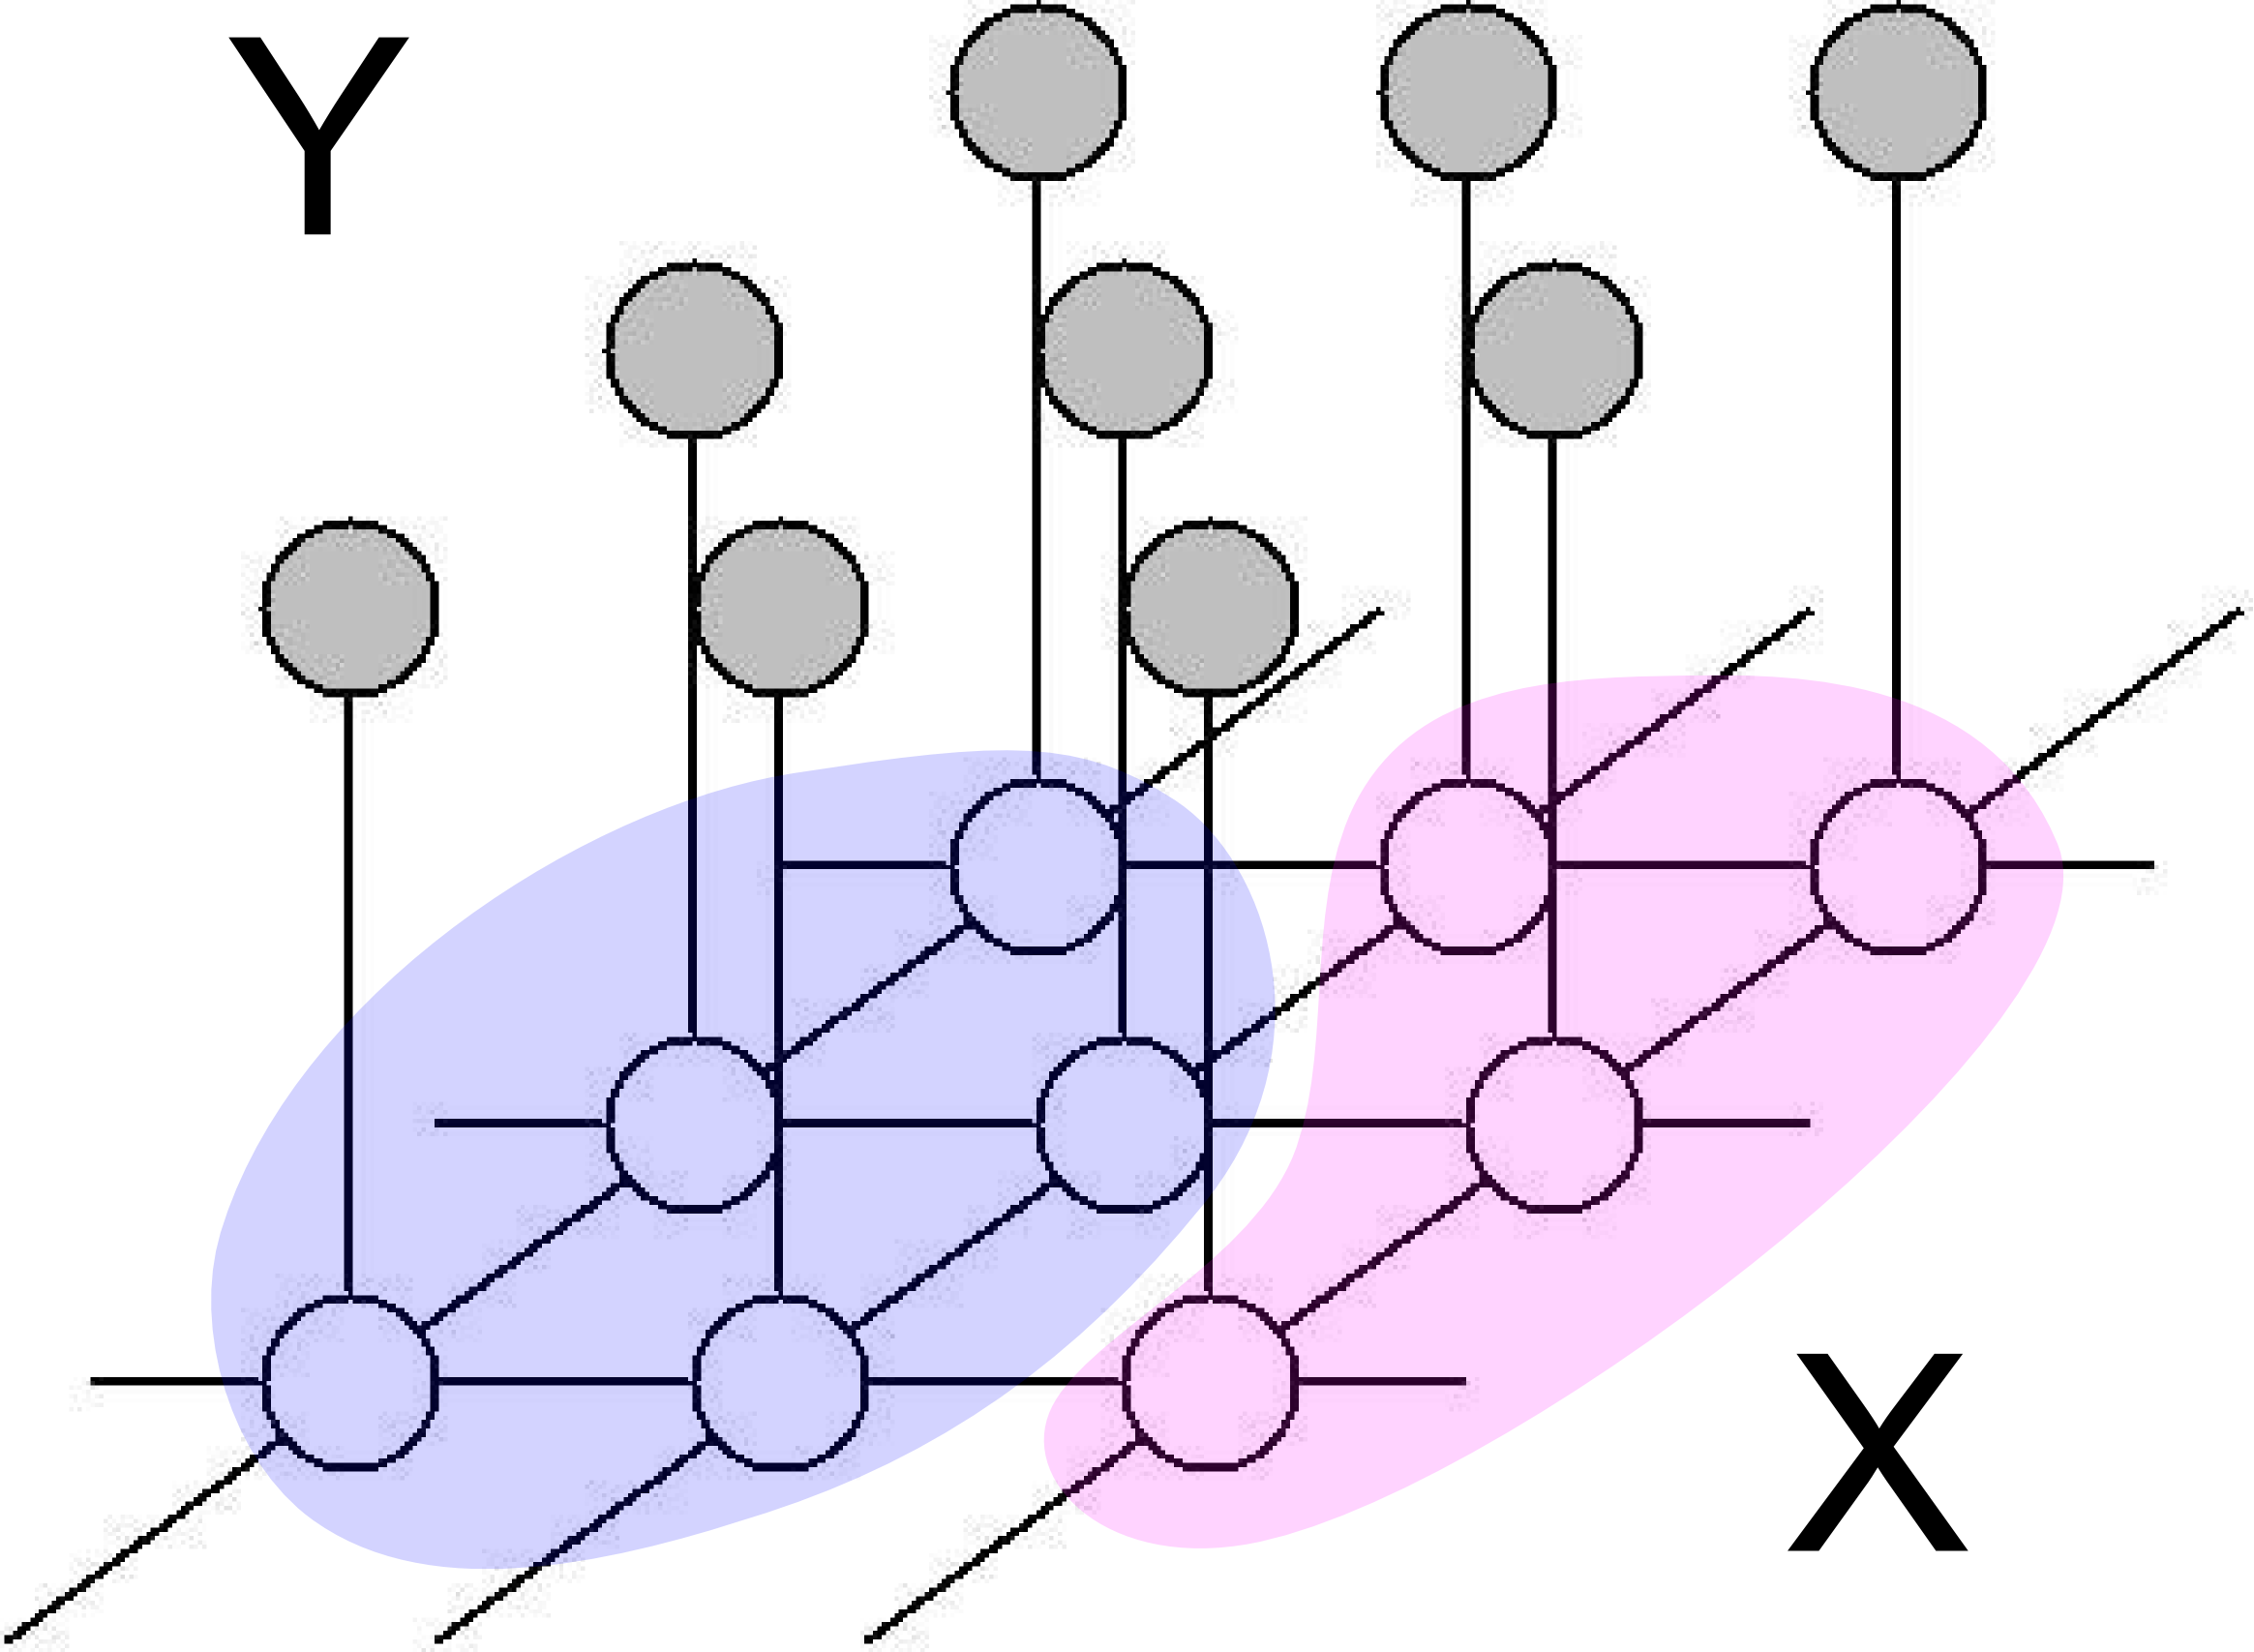
\includegraphics[width=3cm]{sfig/condmrf2a}
    \end{column}
      
  \end{columns}

\end{frame}
%------------------------------------------------------------
\begin{frame}
\frametitle{Full Pairwise Connectivity With Spatial Coherence~\cite{liu2010spatialCopy}}
\begin{block}{The Goal}
  \begin{itemize}
  \item The Connectivity between each pair of voxels.
  \item No Seed region needed.
  \item Spatial smoothness as a regularization, without blurring.
  \item \alert{Learn} the strength of the smoothness from the data.
  \end{itemize}
\end{block}
\end{frame}

\begin{frame}
\frametitle{Full Pairwise Connectivity With Spatial Coherence ~\cite{liu2010spatialCopy} Cont.}
  \begin{columns}
    \begin{column}{7cm}
      \begin{block}{Solution}
        \begin{itemize}
        \item Define a 6 dimension graph $\mathcal{G}$. Define pairwise
          connectivity variable on each node.  Add an edge $(x_{ij}, x_{st})$ if
          any voxels between $i,j$ and $s,t$ are neighbors.
          \item Likelihood: Gaussian $\cN(\mu, \sigma^2)$.
        \item Two class segmentation: no connectivity and connectivity.
        \item Gibbs sampling and mean field approximation to compute posterior mean of X.
        \end{itemize}
      \end{block}
    \end{column}
    \begin{column}{5cm}
      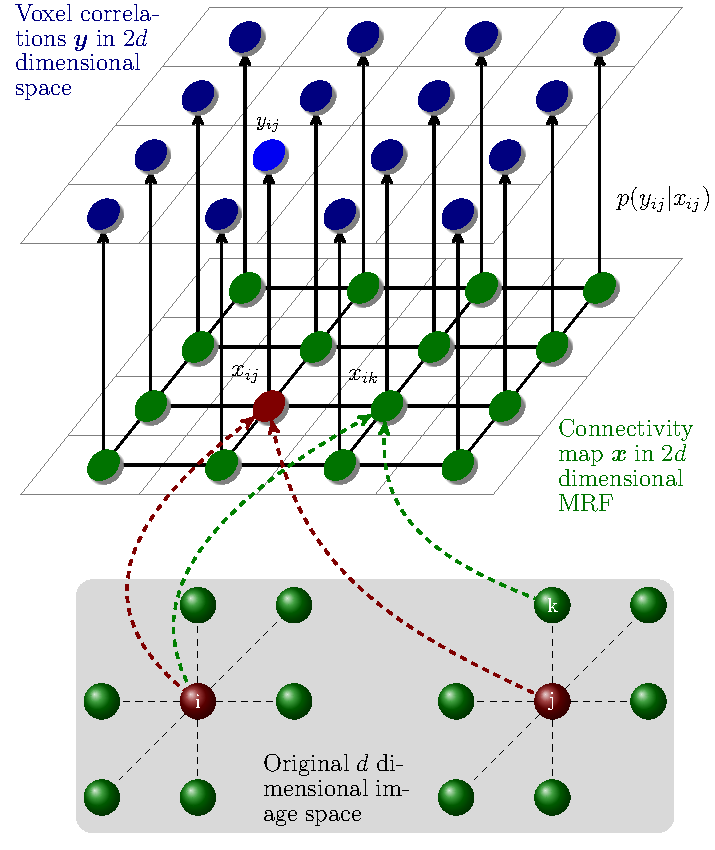
\includegraphics[width=\textwidth]{sfig/6dmrf}
    \end{column}
    \end{columns}
\end{frame}

%--------------------------------------------------------
\begin{frame}
  \frametitle{Experiments on Real data ~\cite{liu2010spatialCopy} }
  \begin{figure}[bth]
    \centering 
      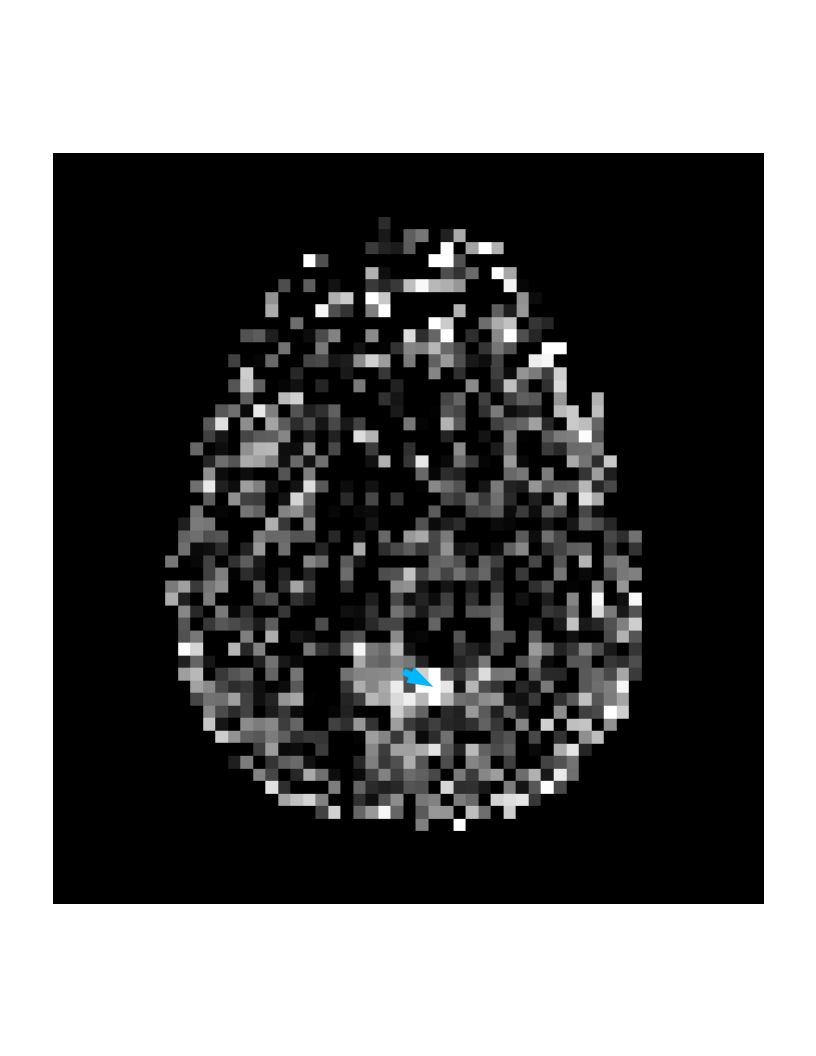
\includegraphics[width = 0.2\textwidth]{figures/no_overlay/R1_corr_nosmooth}
      \hspace{3pt}
      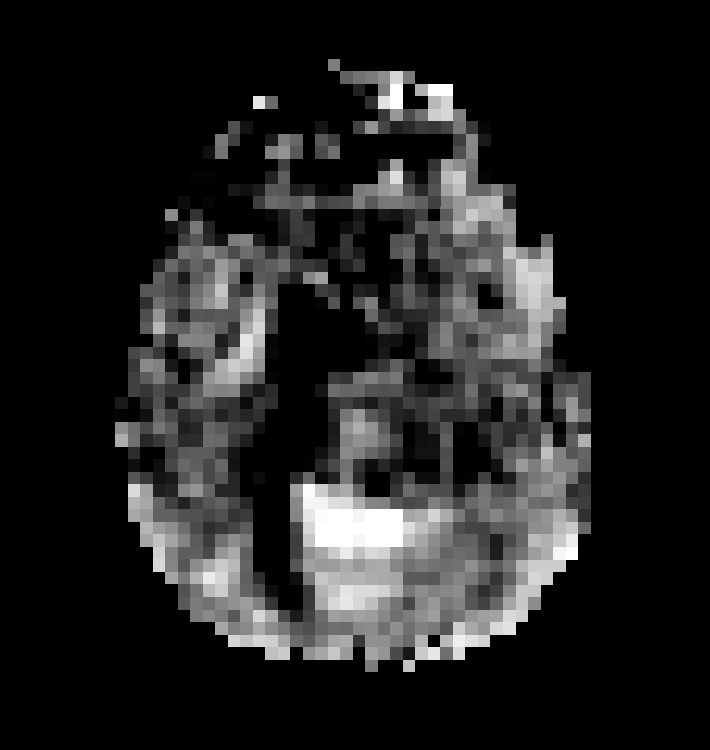
\includegraphics[width = 0.2\textwidth]{figures/no_overlay/R1_corr_smooth}
      \hspace{3pt}
      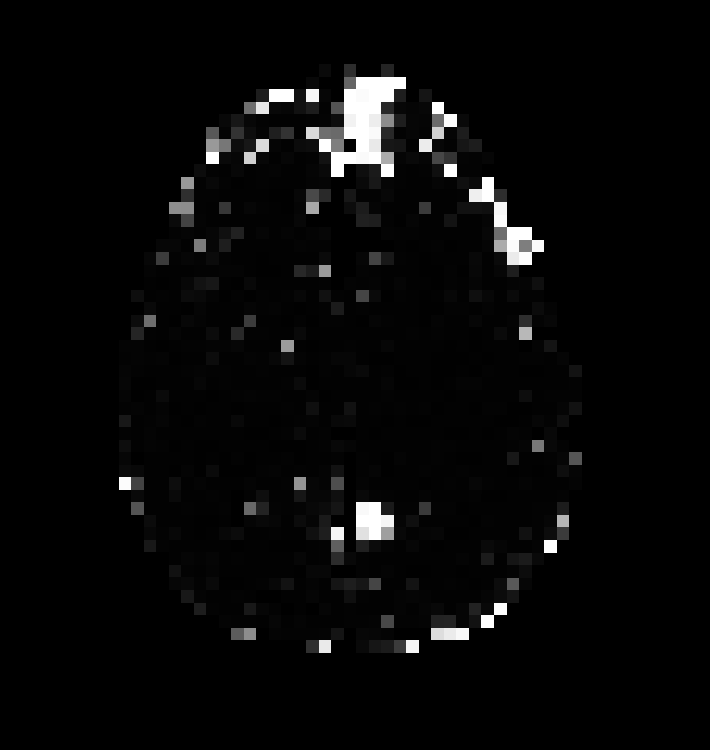
\includegraphics[width = 0.2\textwidth]{figures/no_overlay/R1_mrf} \\
      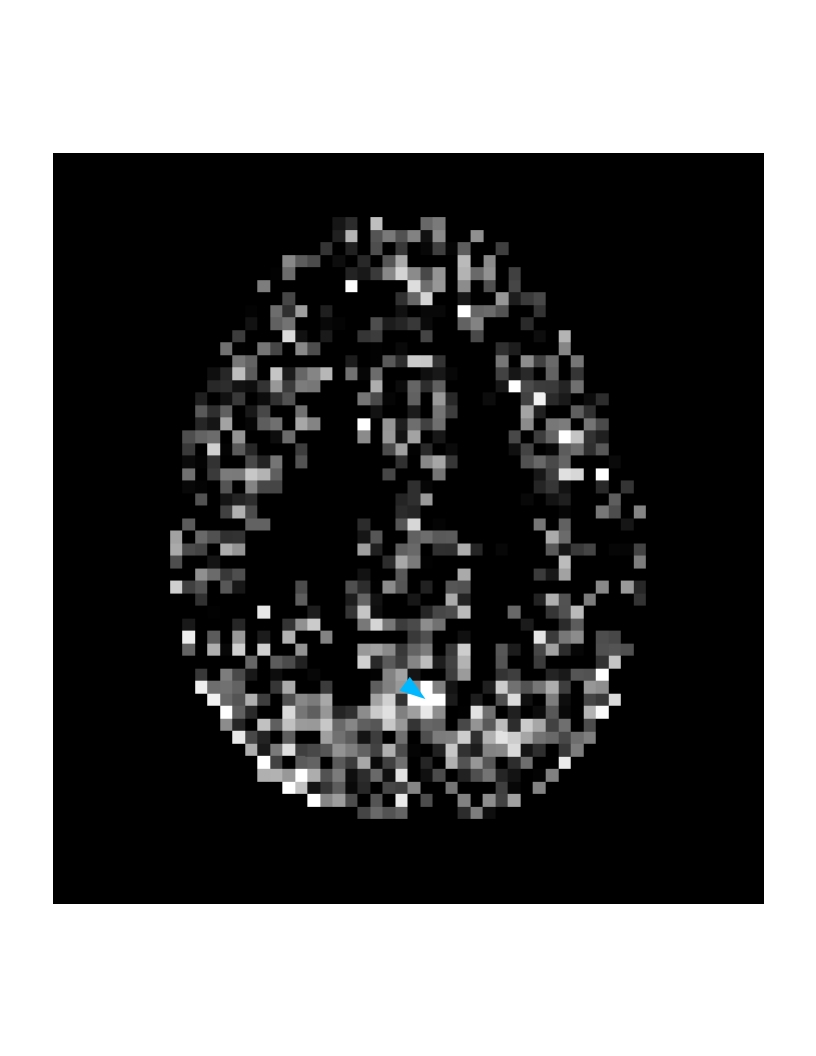
\includegraphics[width = 0.2\textwidth]{figures/no_overlay/R2_corr_nosmooth}
      \hspace{3pt}
      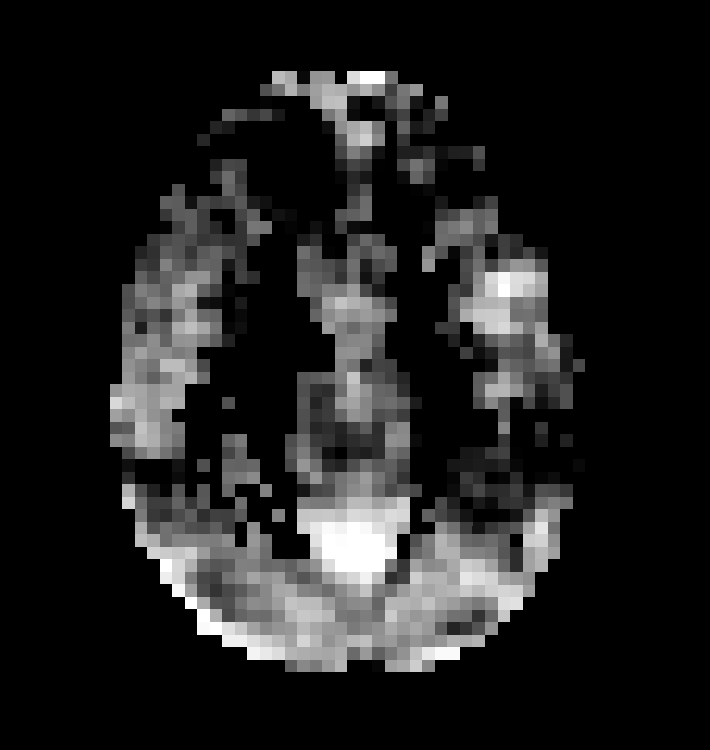
\includegraphics[width = 0.2\textwidth]{figures/no_overlay/R2_corr_smooth}
      \hspace{3pt}
      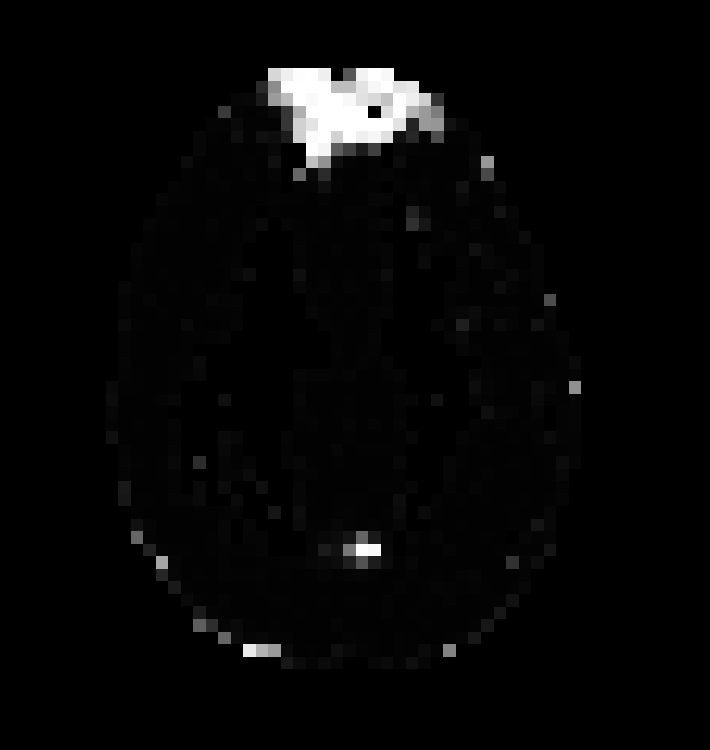
\includegraphics[width = 0.2\textwidth]{figures/no_overlay/R2_mrf}
      \caption{Correlation map without smoothing; With smoothing; Posterior from MRF}
  \end{figure}
  %% \caption{Correlation map and Posterior Connectivity map between
  %%   seed voxel and slice containing the seed. First row is subject
  %%   1. (a) the correlation map computed from data without spatial
  %%   smoothing. (b) correlation map of data after smoothing. (c)
  %%   Posterior probability computed from MRF. Second row (d,e,f) is
  %%   subject 2 with same test.}

\end{frame}
\begin{frame}
\frametitle{Full Pairwise Connectivity With Spatial Coherence Cont.}
  \begin{columns}[c]
    \begin{column}{10cm}
      \begin{block}{Benefits}
        \begin{itemize}
        \item Show functional system real-time once given a seed.
        \item Spatial coherence without over blurring.
        \end{itemize}
      \end{block}
        
      \begin{block}{Issues}
        \begin{itemize}
        \item Can only visualize one functional network.
        \item Big Computation cost.
        \end{itemize}
      \end{block}
    \end{column}

    \end{columns}
\end{frame}
%-------------------------------------------------------
\begin{frame}
\frametitle{Identify Consistent, Spatially Coherent Multiple Functional Networks~\cite{liu2011monteCopy} }
\begin{block}{The Goal}
  \begin{itemize}
  \item Partition the brain into multiple functional networks.
  \item Spatial coherence respected.
  \item Parameter estimation.
  \end{itemize}
\end{block}
\end{frame}

\begin{frame}
\frametitle{Identify Consistent, Spatially Coherent Multiple Functional Networks~\cite{liu2011monteCopy} Cont.}

      \begin{block}{Solution}
        \begin{itemize}
        \item Markov prior $P(X) = \frac{1}{Z} \exp \left ( -\beta \sum_{(r,s)\in \mathcal{E}} \psi(x_s, x_r)\right )$.
        \item Likelihood $P(y_s | X) = C_p(\kappa_l) \exp (\kappa_l \mu_l^{\top} y_s), y_s \in S^{p-1}$.
        \item Inference $P(X | Y) \propto P(X) \cdot P(Y|X) $
        \end{itemize}
      \end{block}

      \includegraphics[width=0.4\textwidth]{sfig/gen}

\end{frame}

\begin{frame}
\frametitle{Identify Consistent, Spatially Coherent Multiple Functional Networks ~\cite{liu2011monteCopy} Cont.}

\begin{block}{Expectation Maximization}
  \begin{equation*}
    Obj = \mathbb{E}_{X|Y} [\log P(X,Y;\theta)]
  \end{equation*}
\end{block}

\begin{block}{Monte Carlo Expectation Maximization}
  \begin{equation*}
    \mathbb{E}_{X|Y} [\log P(X,Y;\theta)] \approx \frac{1}{M}\sum_m \log P(X^m; \theta) + \log P(Y|X^m; \theta)
  \end{equation*}
\end{block}

\begin{block}{Pseudo Likelihood}

  \begin{equation*}
    \log P(X^m; \theta) \approx \sum_{s\in \mathcal{V}} \log P(x_s | x_{\mathcal{N}_s};\theta)
  \end{equation*}
\end{block}
\end{frame}
%------------------------------------------
\begin{frame}
\frametitle{Identify Consistent, Spatially Coherent Multiple Functional Networks Cont.}
\begin{figure}[htb]
 \begin{center}
 \begin{tabular}{cccccc}
      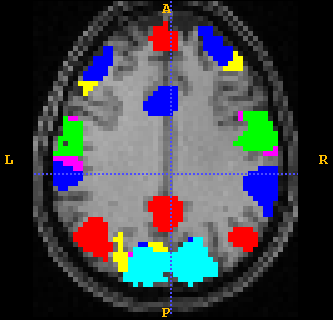
\includegraphics[width=0.12\textwidth]{figures/wholebrain/sub1/axial0028} &
      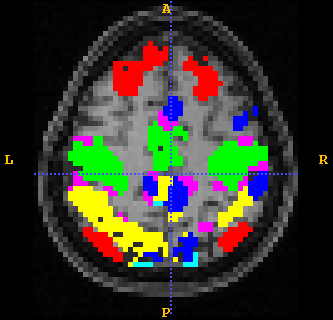
\includegraphics[width=0.12\textwidth]{figures/wholebrain/sub1/axial0034} &
      %% \vspace{0.5pt}
      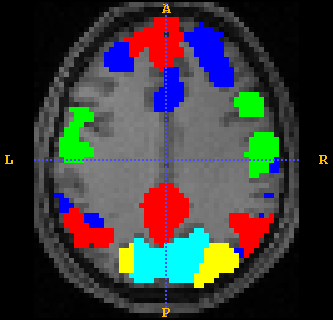
\includegraphics[width=0.12\textwidth]{figures/wholebrain/sub2/axial0028} &
      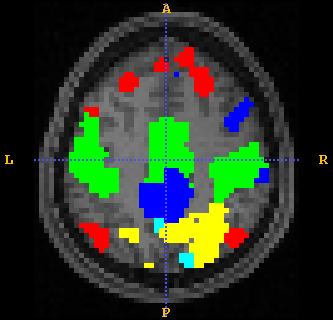
\includegraphics[width=0.12\textwidth]{figures/wholebrain/sub2/axial0034} &
      %% \vspace{0.5pt}
      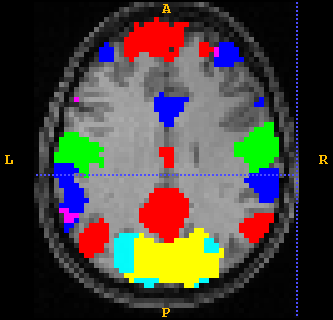
\includegraphics[width=0.12\textwidth]{figures/wholebrain/sub5/axial0028} &
      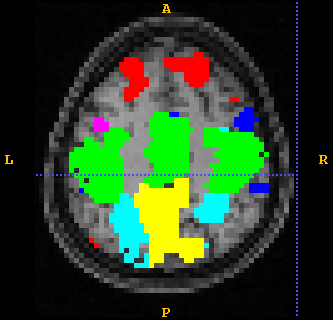
\includegraphics[width=0.12\textwidth]{figures/wholebrain/sub5/axial0034} \\

      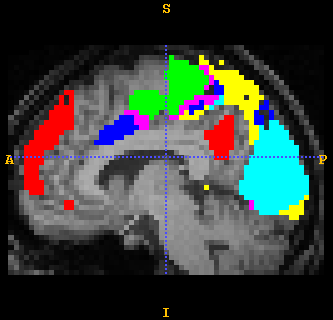
\includegraphics[width=0.12\textwidth]{figures/wholebrain/sub1/saggital0029} &
      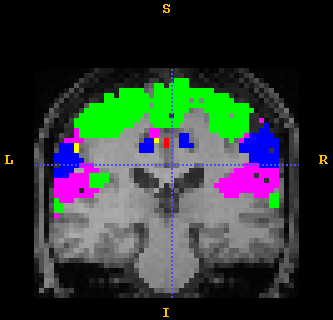
\includegraphics[width=0.12\textwidth]{figures/wholebrain/sub1/coronal0029} &
      %% \vspace{0.5pt}

      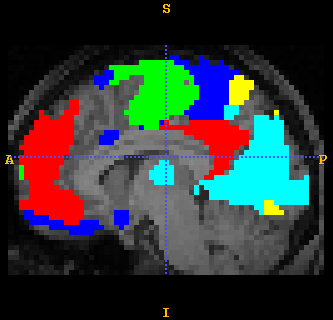
\includegraphics[width=0.12\textwidth]{figures/wholebrain/sub2/saggital0029} &
      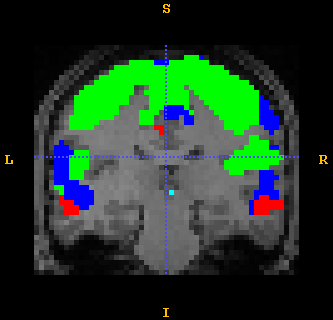
\includegraphics[width=0.12\textwidth]{figures/wholebrain/sub2/coronal0029} &
      %% \vspace{0.5pt}
      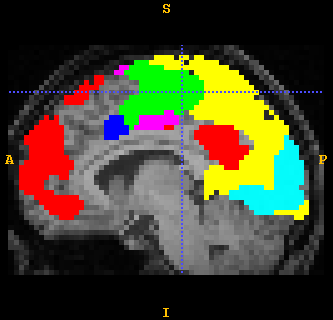
\includegraphics[width=0.12\textwidth]{figures/wholebrain/sub5/saggital0029} &
      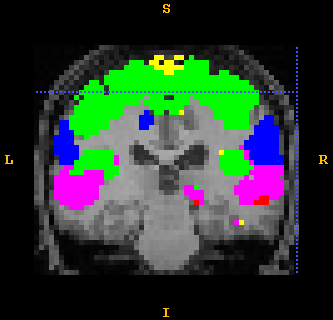
\includegraphics[width=0.12\textwidth]{figures/wholebrain/sub5/coronal0029}\\

      \multicolumn{2}{c}{\small Subject 1} &
      \multicolumn{2}{c}{\small Subject 2} &
      \multicolumn{2}{c}{\small Subject 3}
    \end{tabular}
  \end{center}
  %% \caption {Functional networks detected by the proposed method for 3 subjects
  %%   overlaid on their T1 images.  The clusters are the visual (cyan), motor
  %%   (green), executive control (blue), salience (magenta), dorsal attention
  %%   (yellow), and default mode (red) networks.}
\end{figure}
\end{frame}
%---------------------------------------------
\begin{frame}
\frametitle{Current Work: Hierarchical Model For Group Study~\cite{Liu2012aCopy} }
\begin{block}{Goal}
  \begin{itemize}
    \item A Bayesian approach for group analysis.
    \item Both group and subject functional networks are identified.
    \item Group and subjects use each other as priors for a joint optimal solution.
  \end{itemize}
\end{block}
\end{frame}
%----------------------------------------------------
\begin{frame}
\frametitle{State-of-Art Group Analysis Approach}
\vspace{-10pt}
\begin{columns}[t]
  \begin{column}{5.5cm}
    \begin{block}{Bottom-up Approach (Heuvel, 2008; Craddock, HBM, 2011)}
      \begin{itemize}
        \item Estimate Subject network first.
        \item Estimate group network from subjects.
      \end{itemize}
    \end{block}
    %% \vspace{10pt}
    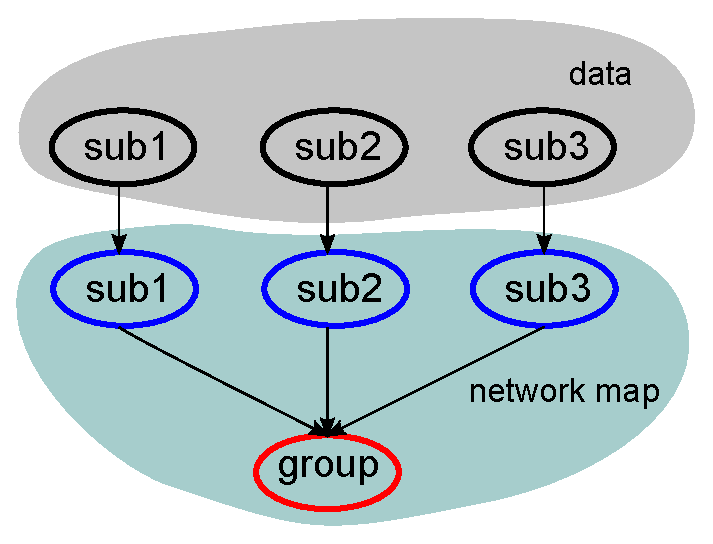
\includegraphics[width=\textwidth]{sfig/hier1}
  \end{column}

  \begin{column}{5.5cm}
    \begin{block}{Top-down Approach (Calhoun, HBM, 2001)}
      \begin{itemize}
        \item Estimate group network from all subjects.
        \item Back-reconstruct  subject network maps.
      \end{itemize}
    \end{block}
    %% \vspace{10pt}
    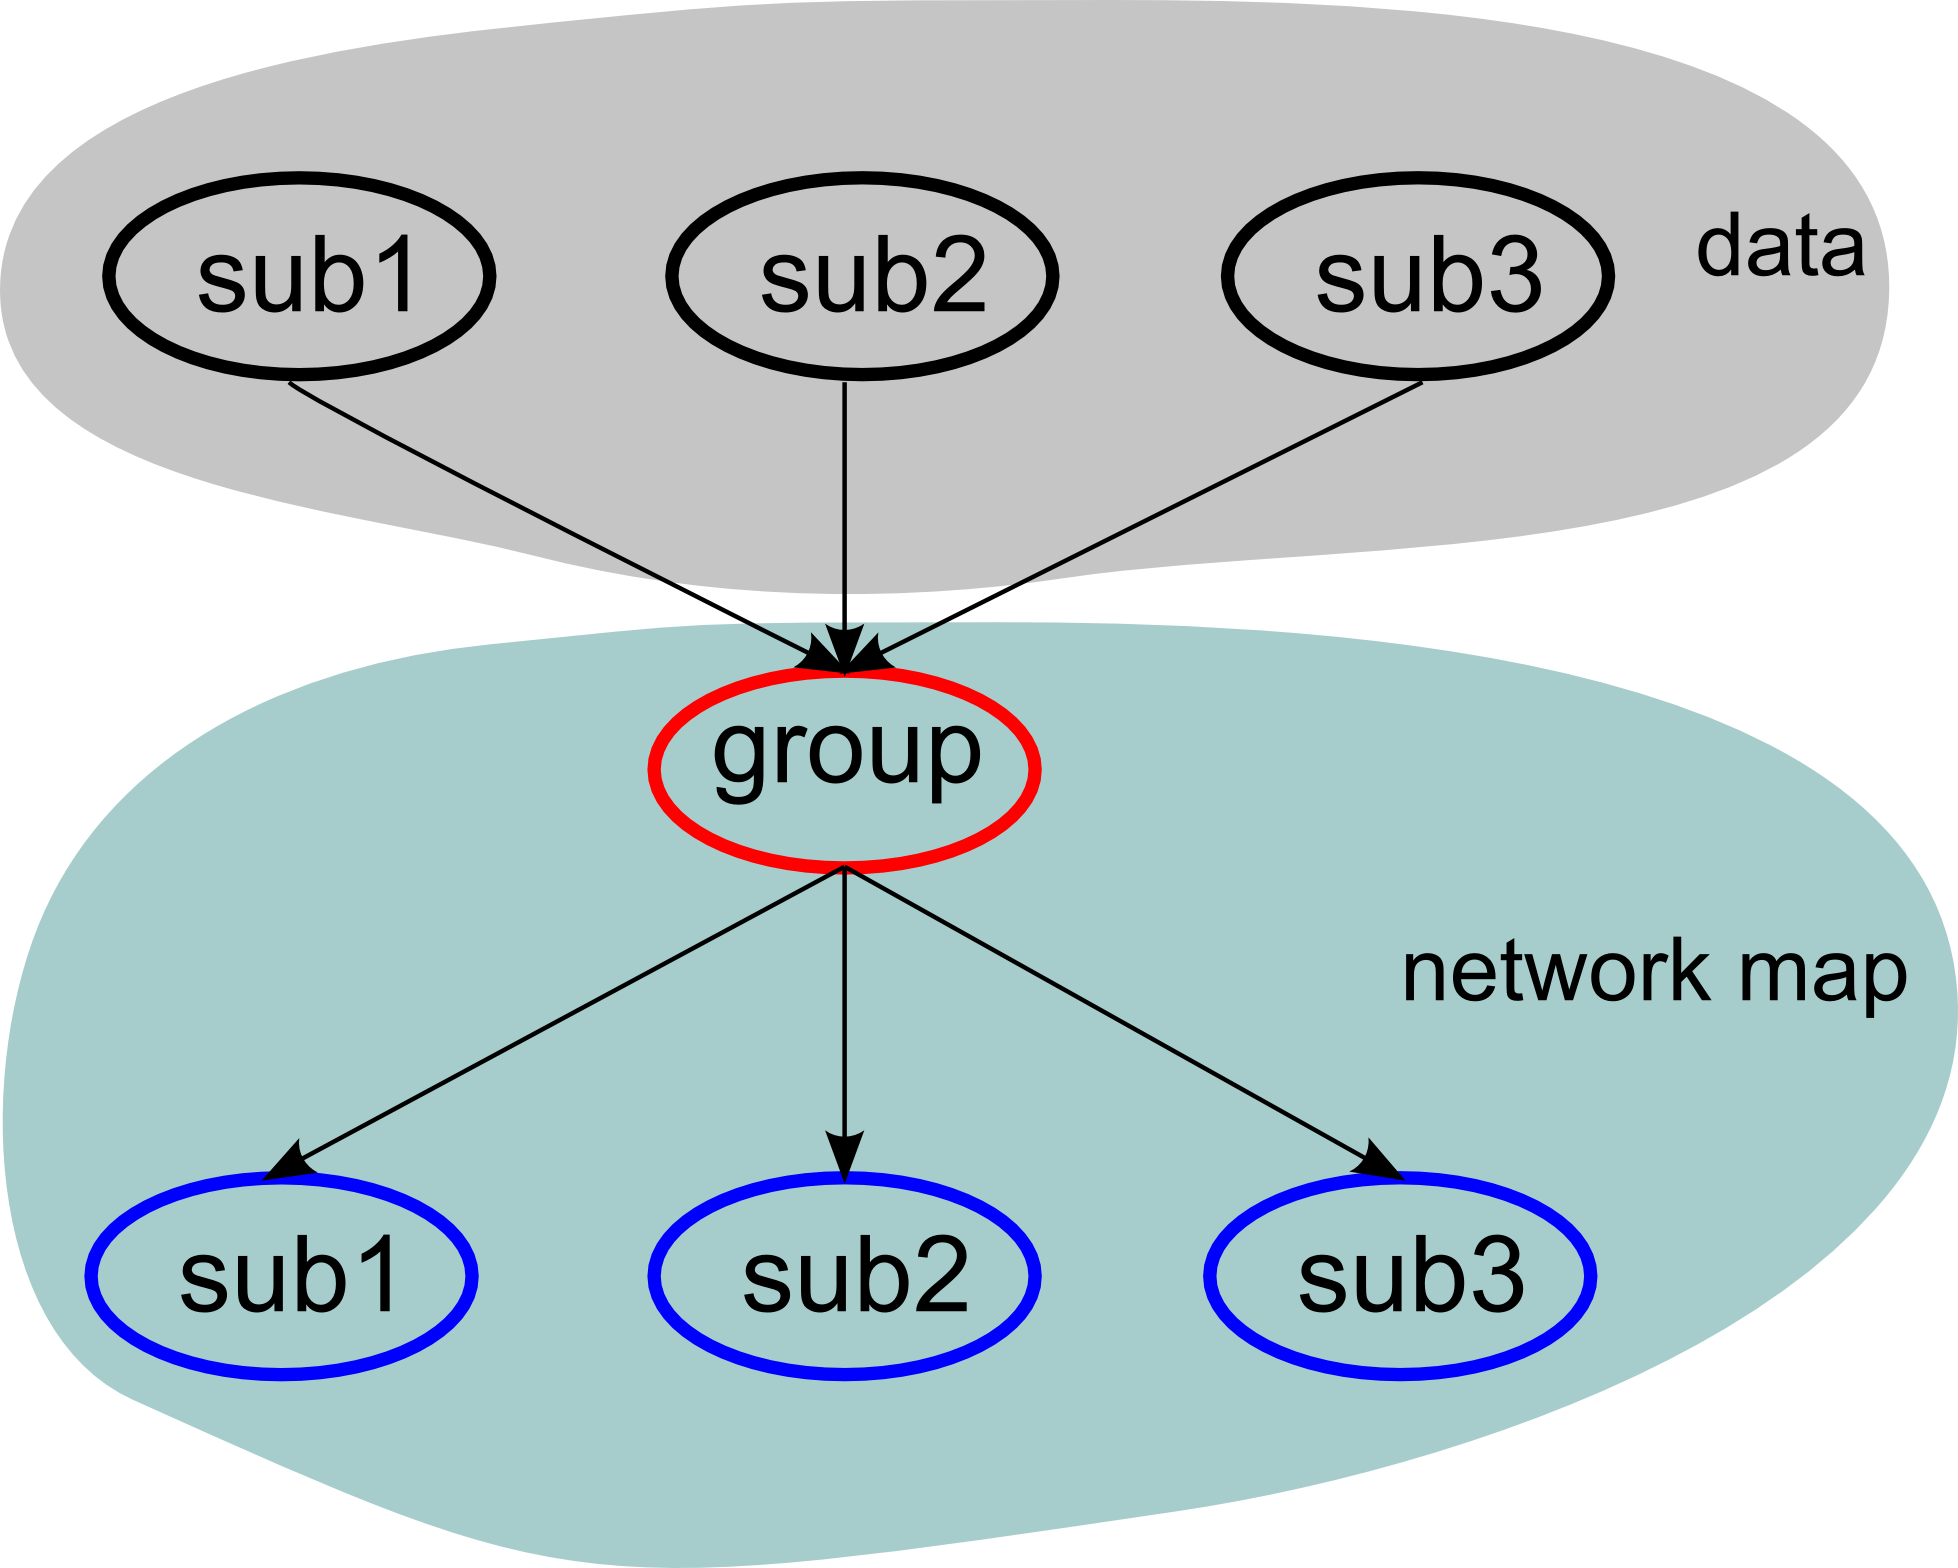
\includegraphics[width=\textwidth]{sfig/hier2}
  \end{column}
\end{columns}
\end{frame}

\begin{frame}
  \frametitle{Joint Estimation: a Better Approach~\cite{Liu2012aCopy} }
  \begin{columns}
    \begin{column}{5cm}
        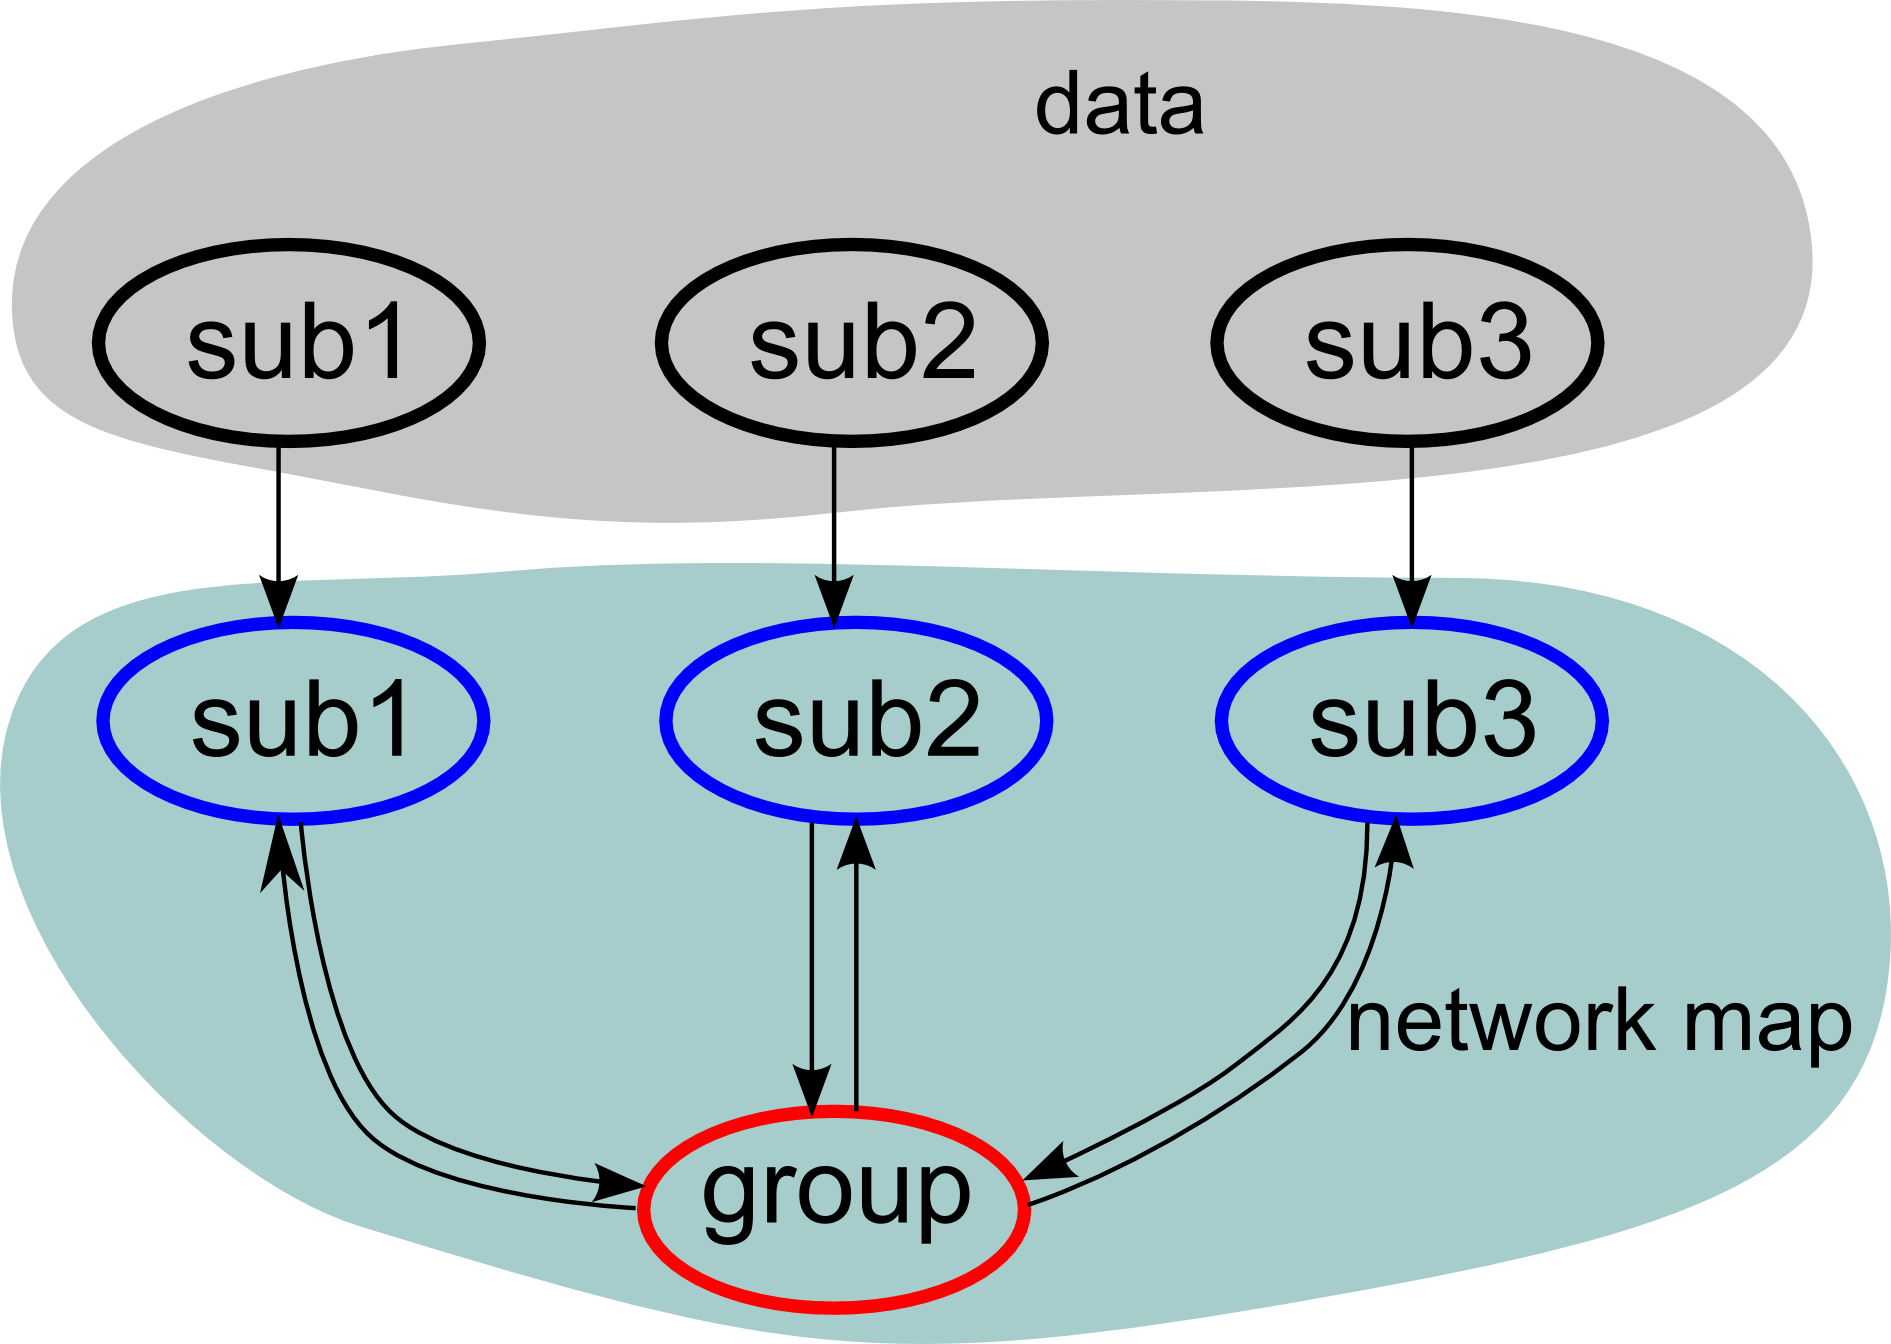
\includegraphics[width=\textwidth]{sfig/hier3}
    \end{column}

    \begin{column}{5cm}
      \begin{block}{}
        \begin{itemize}
          \item Group network map inform subjects as a prior.
          \item Subject network maps feedback into group estimation.
          \item Jointly estimate both levels.
        \end{itemize}
      \end{block}
    \end{column}
    
  \end{columns}
\end{frame}

\begin{frame}
  \frametitle{Joint Estimation With MRF}
  \begin{block}{}
    Spatial coherence is again modeled by MRF.
  \end{block}
  \vspace{10pt}
  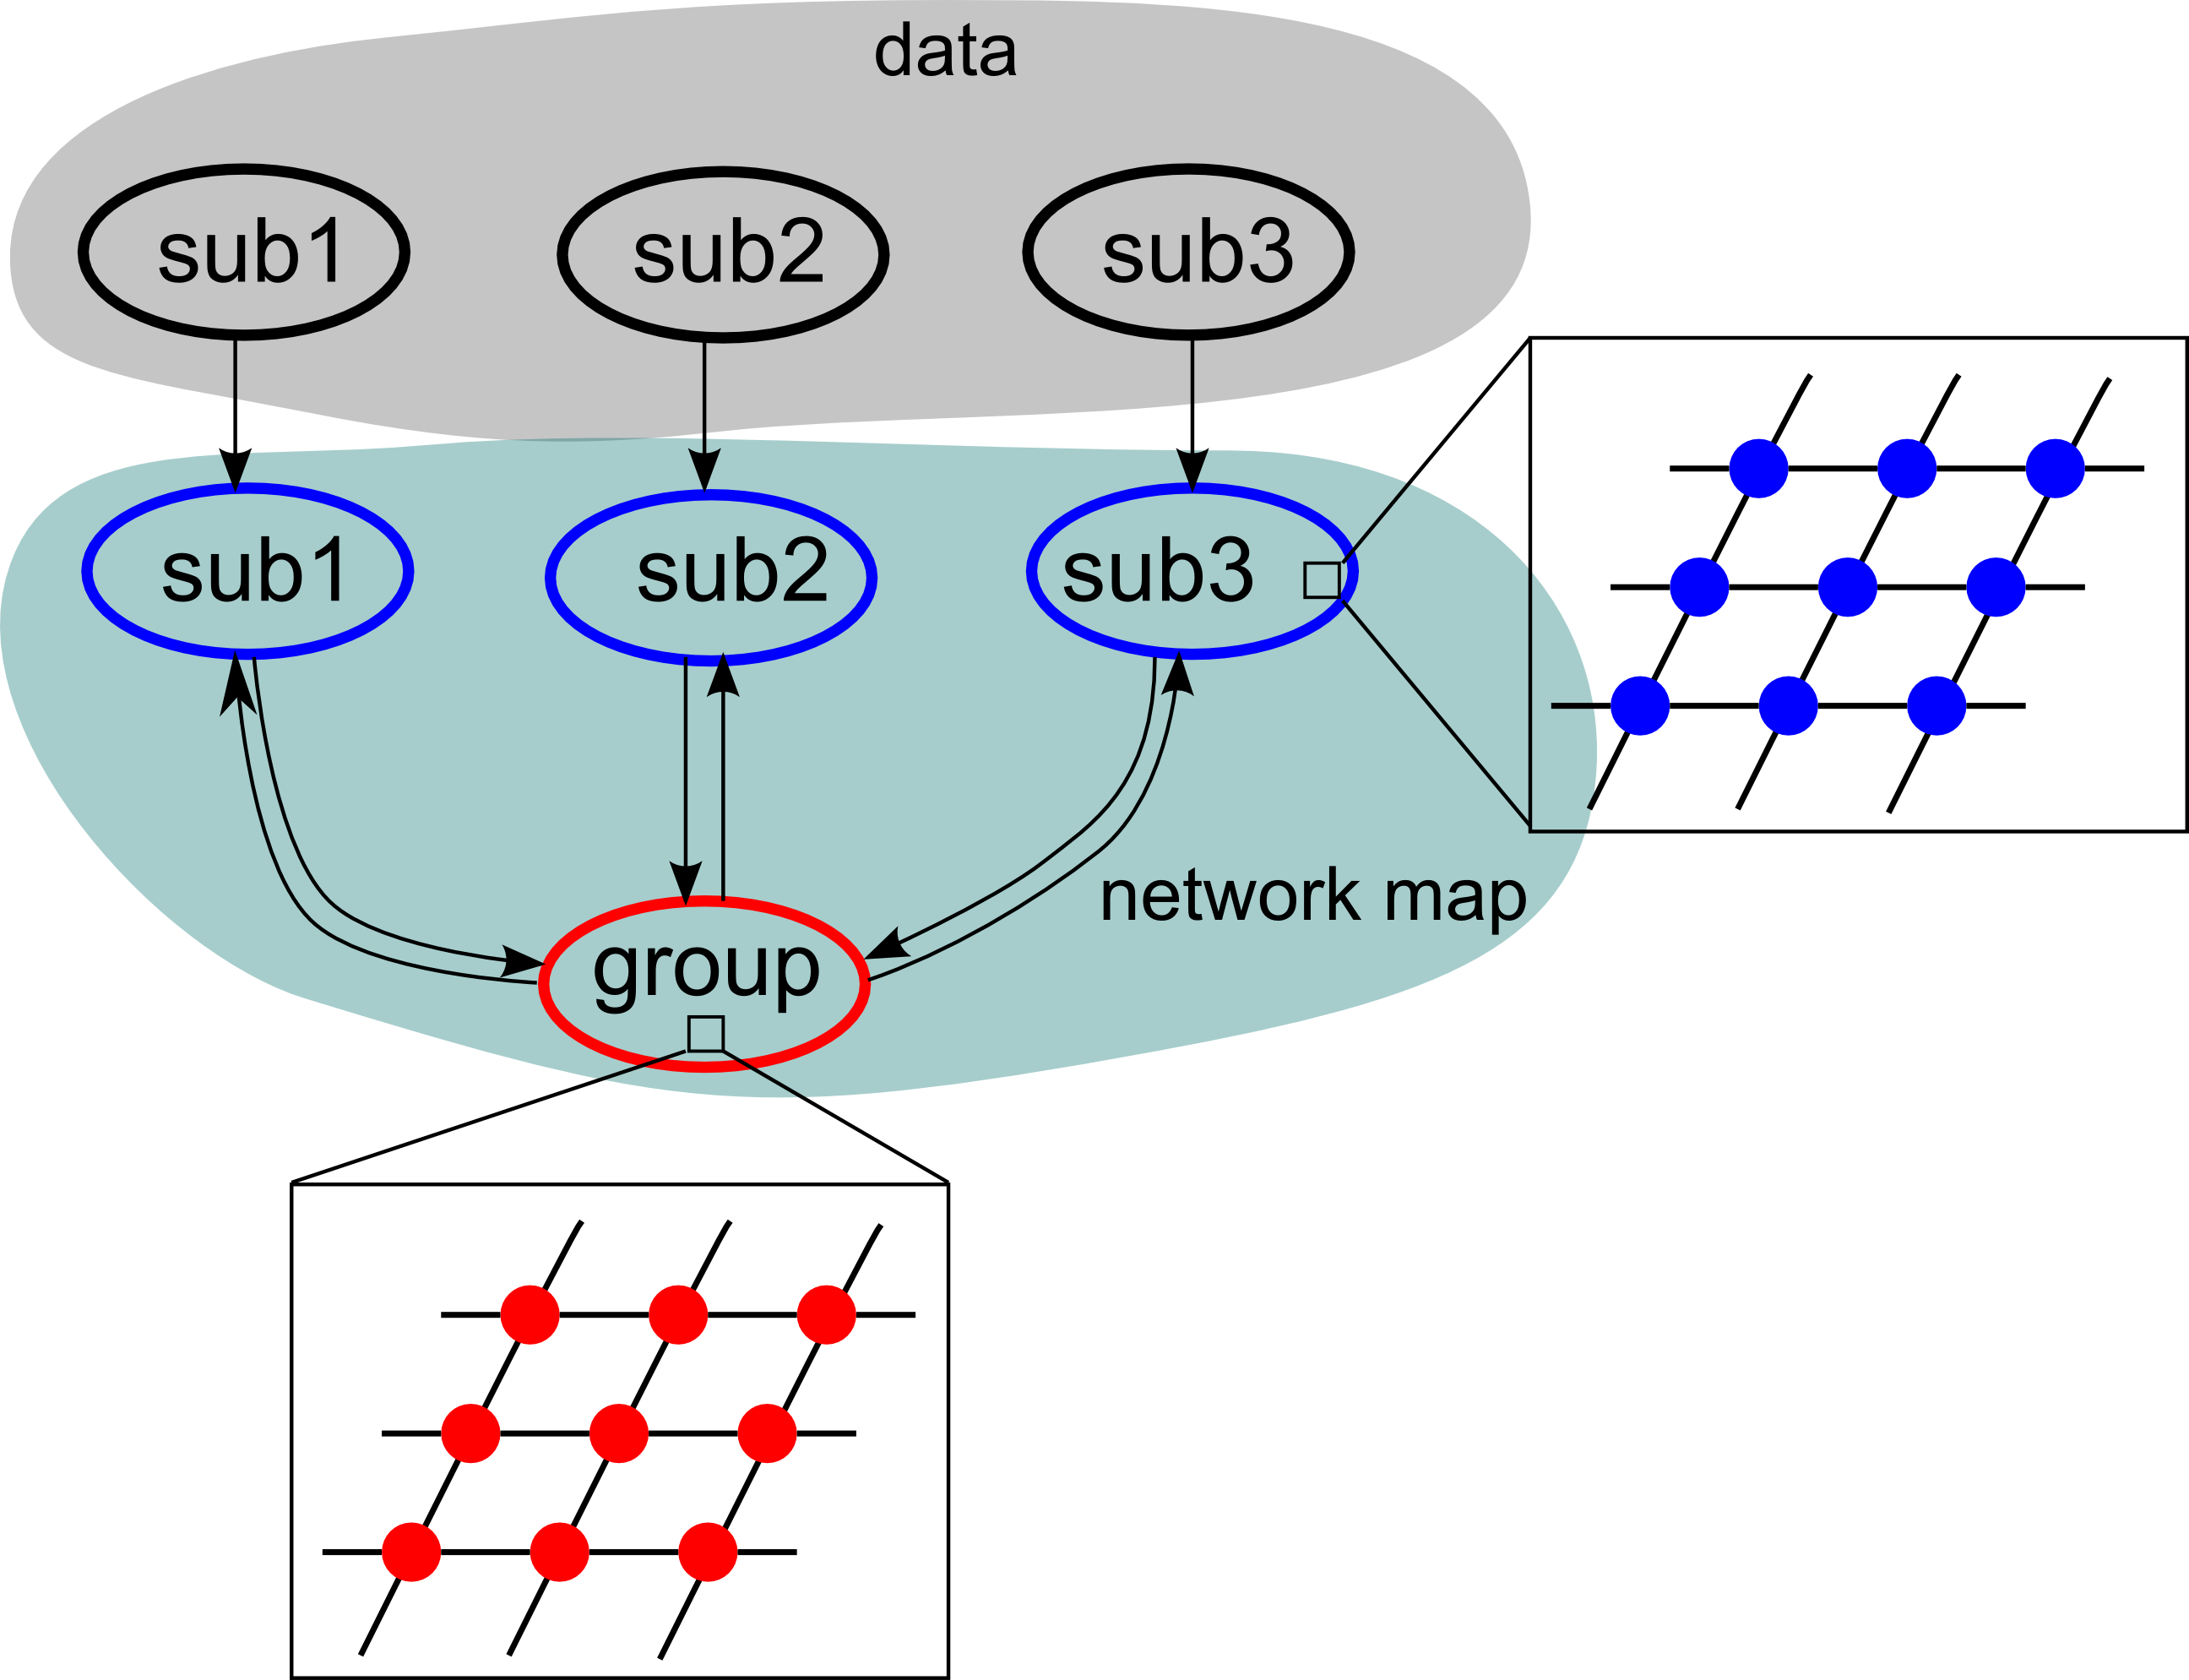
\includegraphics[width=0.7\textwidth]{sfig/hier3a}
\end{frame}


\begin{frame}
  \frametitle{A new MRF including both levels}
  \begin{columns}
    \begin{column}{5cm}
      \begin{block}{}
        Put group and all subject network label variables in a single graph.
      \end{block}
    \end{column}

    \begin{column}{6cm}
    \includegraphics[width=0.8\textwidth]{figure1/grp2}
    \end{column}
  \end{columns}
\end{frame}

%----------------------------------------------------
\begin{frame}
  \frametitle{MRF Prior of The New Graph}
  \begin{columns}
    \begin{column}{7.5cm}  
      \begin{definition}
        $\cG_G = (\cV_G, \cE_G)$: Graph that represents group map.\\
        $\cG_H^j = (\cV_H^j, \cE_H^j), \forall j = 1, \dots, J$: subject map. \\
        $\cG=(\cV, \cE)$: new graph that includes both group and subject level. \\
        $\cV = (\cV_H, \cV_H^1, \dots, \cV_H^J)$, $\cE = \{(r,s) | (r,s) \in \cE_G\} \cup \{(r,s) | r \in \cV_G, s\in \cV_H^j, r\simeq s\} \cup \{(r,s) | (r,s) \in \cE_H^j\}$.
      \end{definition}
    \end{column}

    \begin{column}{4cm}
      \includegraphics[width=0.8\textwidth]{figure1/grp2}
    \end{column}
  \end{columns}
\end{frame}

%----------------------------------------------------
\begin{frame}
  \frametitle{MRF Prior of The New Graph}
  \begin{columns}
    \begin{column}{8cm}  

      \begin{block}{Energy Function}
        \begin{align*}
          U(X) &= \sum_{(s,r)\in\cE_H} \beta \psi(x_s, x_r) \\
          &+ \sum_{j=1}^J \left ( \sum_{s\in\cV_G, \tilde s\in\cV_H^j} \alpha \psi(x_s, x_{\tilde s}) \right.\\
          &\left.+ \sum_{(s,r)\in\cE_H^j}\beta\psi(x_s, x_r) \right ).
        \end{align*}
      \end{block}

    \end{column}

    \begin{column}{3cm}
      \includegraphics[width=\textwidth]{figure1/grp2}
    \end{column}
  \end{columns}
\end{frame}
%-----------------------------------------------


\begin{frame}
  \frametitle{Likelihood}
  \begin{columns}[c]
    \begin{column}{3cm}
      \includegraphics[width=\textwidth]{figure1/grp2}
    \end{column}

    \begin{column}{7cm}
      \begin{block}{}
        $y_s$: normalized time series in p-sphere.
      \end{block}

      \begin{block}{Likelihood}
        \begin{equation*}
          P(y_s | X) = C_p(\kappa_l) \exp (\kappa_l \mu_l^{\top} y_s), y_s \in S^{p-1}.
        \end{equation*}

        \begin{equation*}
          \log P(Y|X) = \sum_{s\in H} \log p(y_s | x_s)
        \end{equation*}
      \end{block}
    \end{column}
  \end{columns}

\end{frame}

\begin{frame}
  \frametitle{Bayesian Inference: Gibbs Sampling}
  \begin{block}{}
    \begin{itemize}
      \item Monte-Carlo Sampling used to approximate $\mathbb{E}_{X|Y} [\log
        P(X,Y;\theta)]$
        \item Gibbs sampling also in a multi-level fashion.
    \end{itemize}
    \end{block}
  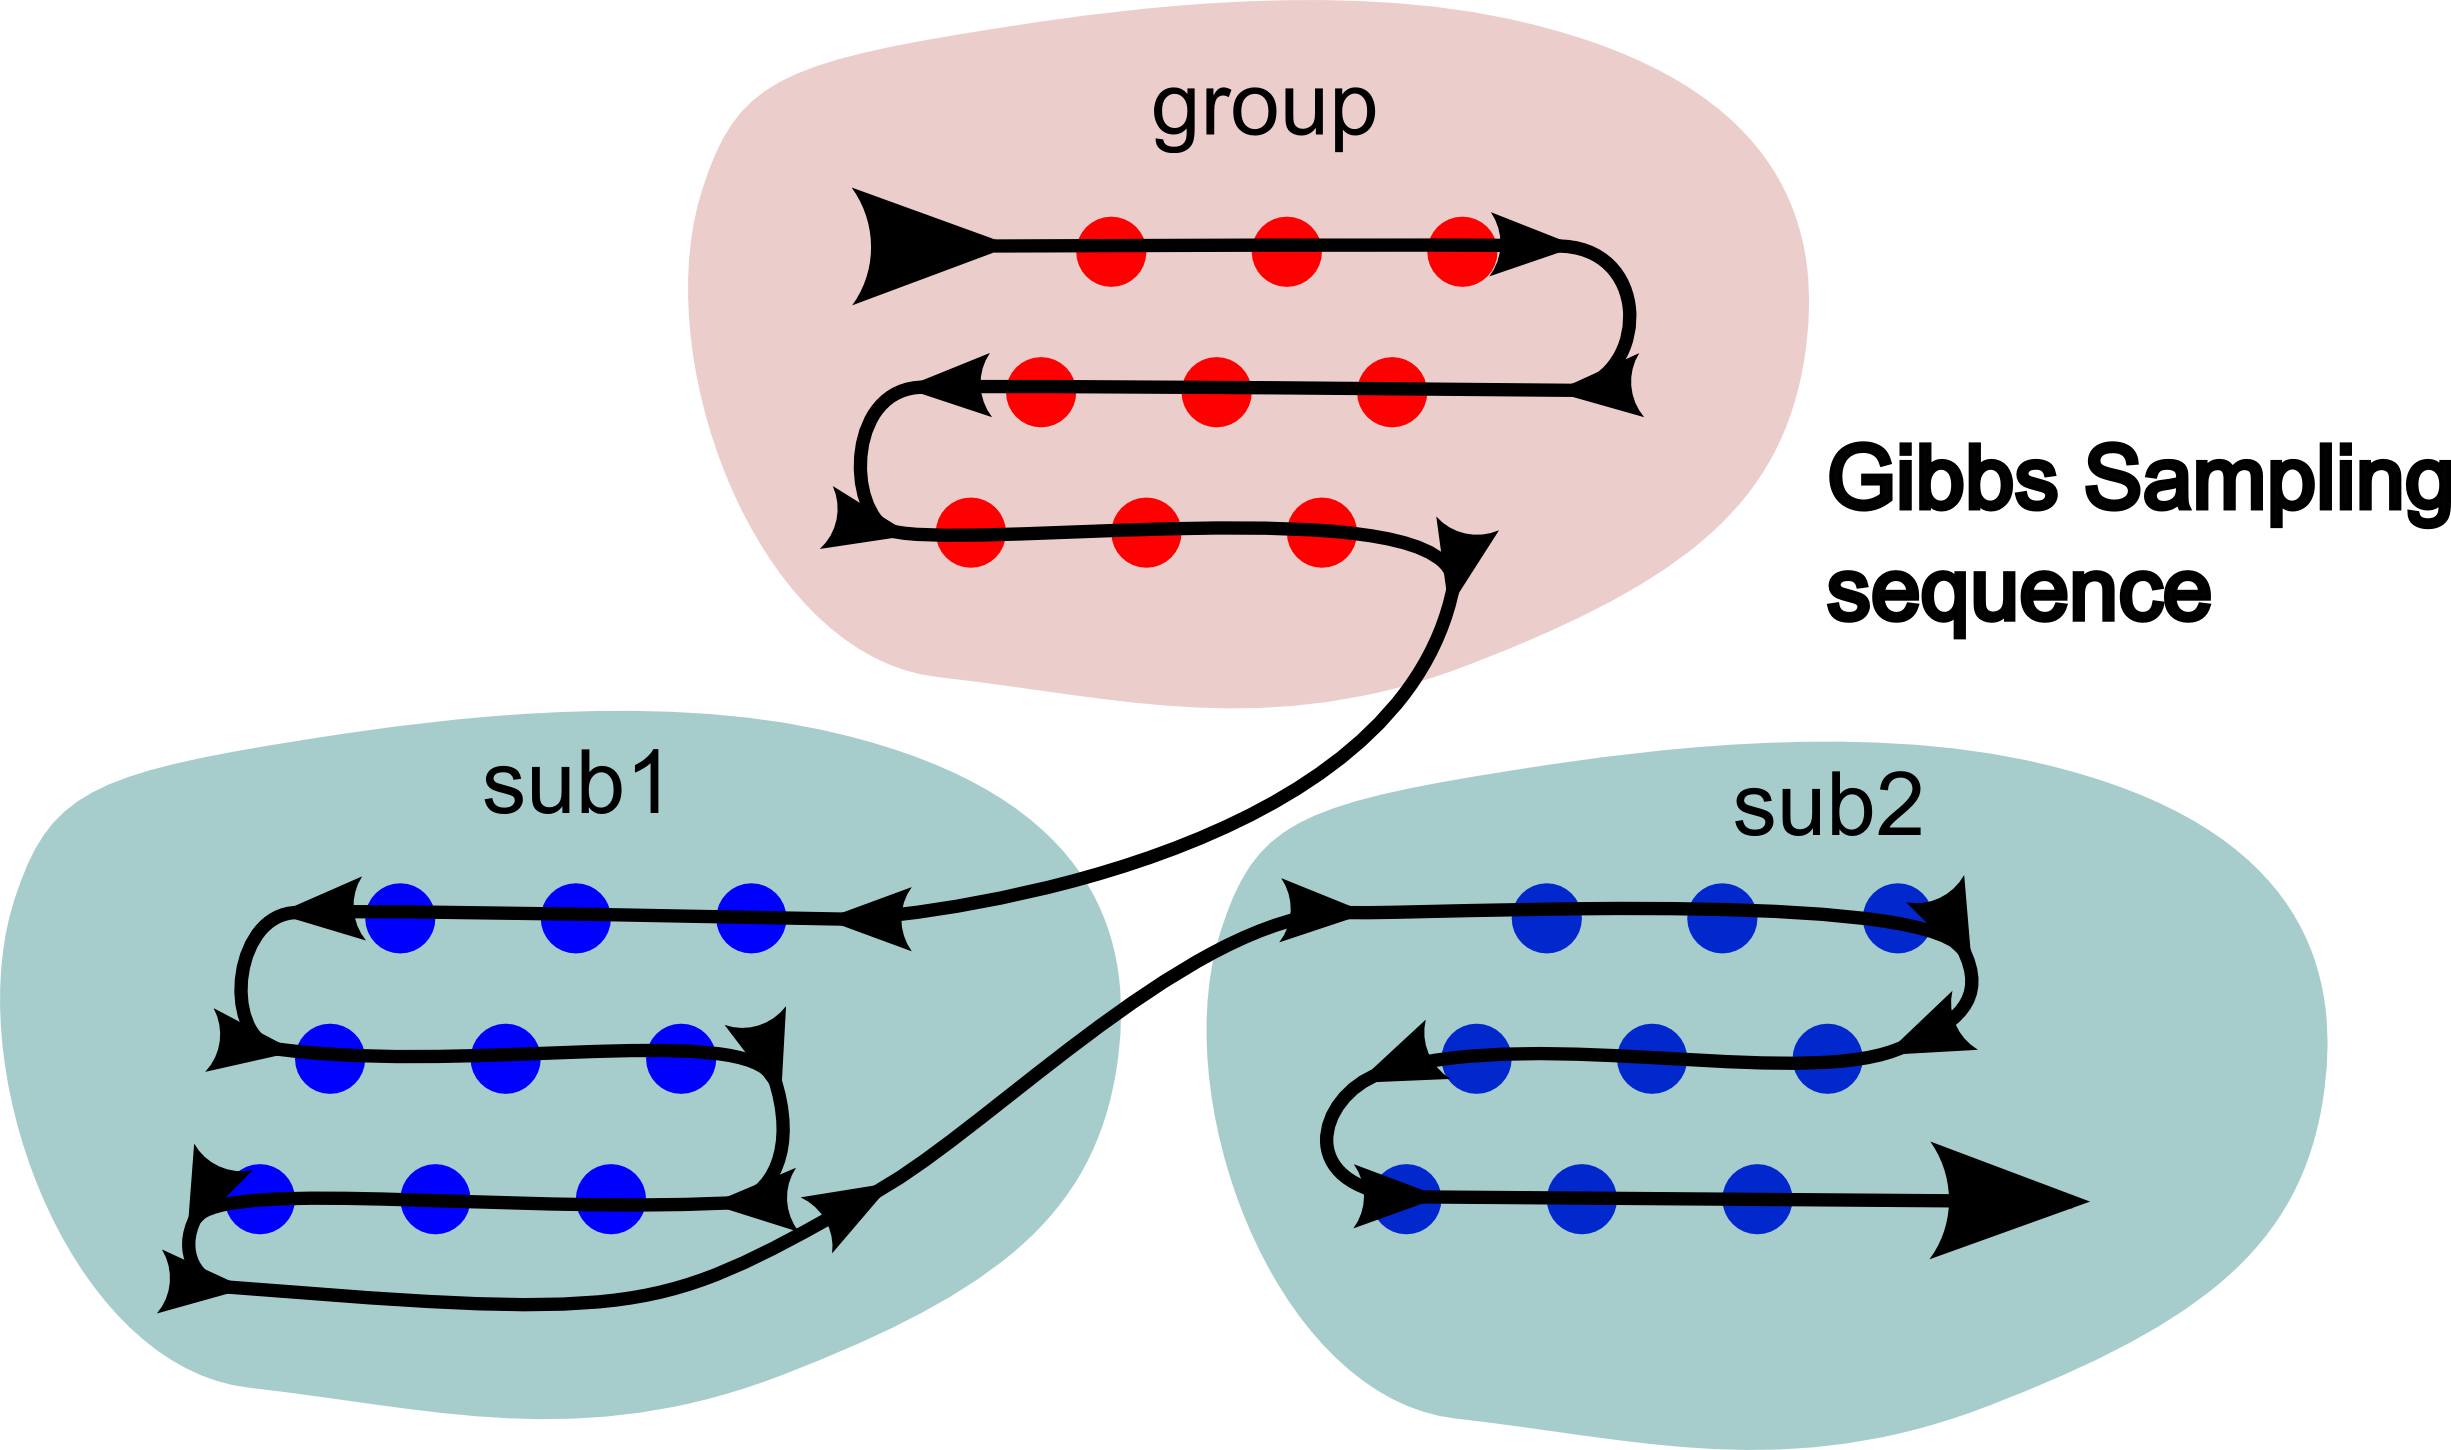
\includegraphics[width=0.7\textwidth]{sfig/hiergibbs2}
\end{frame}


\begin{frame}
\frametitle{The Algorithm}
\begin{algorithm}[H]
  \label{alg:alg1}
  %% \SetAlgoLined
  \KwData{Normalized fMRI, initial group label map}
  \KwResult{Group and subjects label map $X$, parameters $\{\alpha, \beta, \mu, \sigma\}$}
  \While{$\mathbb{E}[\log p(X, Y)]$ not converge}{
    %% E step\;
    \Repeat{$B+M$ times}{
      \lForEach(){$s \in \cV_G$}{
        Draw consecutive samples of $x_s$
      }
      \ForEach(){$j  = 1\dots J$}{
        \lForEach(){$s \in \cV_H^j$}{
        Draw consecutive samples of $x_s$
        }
      }
      Save sample $Y^m $ after $B$ burn-ins\;
    }
    %% M step\;
    \lForEach{$l = 1\cdots L$} {
      Estimate $\{\mu_l, \kappa_l\}$ by maximizing $\frac{1}{M}\sum_{m=1}^M\log p (Y|X^m)$\;
    }
    Estimate $\{\alpha, \beta\}$ by maximizing $\frac{1}{M}\sum_{m=1}^M\log p (X^m)$\;
  }
  Run ICM on current samples to estimate final label maps.
\end{algorithm}
\end{frame}

\begin{frame}
\frametitle{Synthetic Data Experiment}
\begin{figure}[htb]
  \begin{tabular}[b]{c}
    \begin{tabular}[b]{lccccc}
      & \footnotesize Truth & \footnotesize \textsf{K-Means} & \footnotesize \textsf{N-Cuts} & \footnotesize \textsf{groupmrf}\\
      \begin{sideways} \footnotesize group \end{sideways} &
      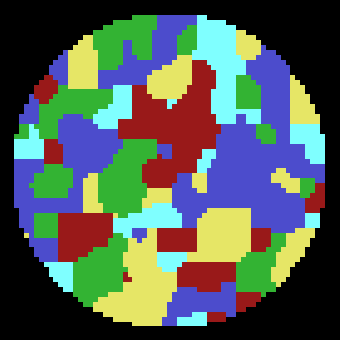
\includegraphics[width=0.12\textwidth]{figure1/truegrp} &
      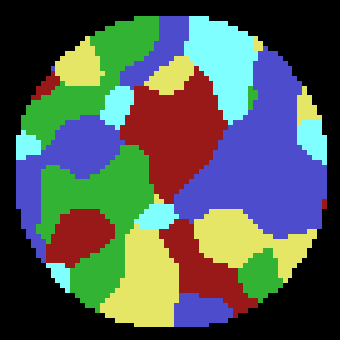
\includegraphics[width=0.12\textwidth]{figure1/kmeans_grp} &
      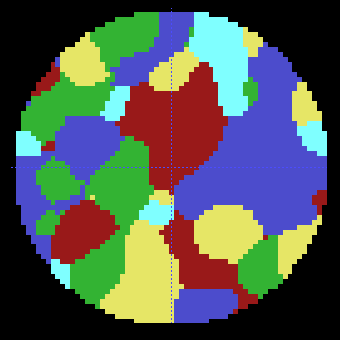
\includegraphics[width=0.12\textwidth]{figure1/ncuts_grp} &
      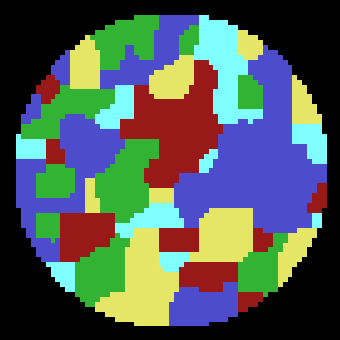
\includegraphics[width=0.12\textwidth]{figure1/mrf_grp} \\
      \begin{sideways} \footnotesize sub 1 \end{sideways} &
      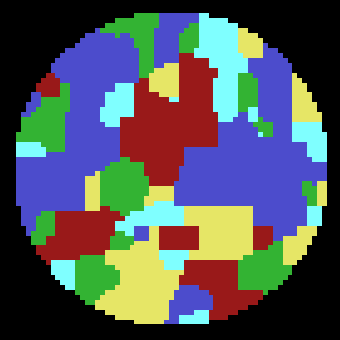
\includegraphics[width=0.12\textwidth]{figure1/true_sub1} &
      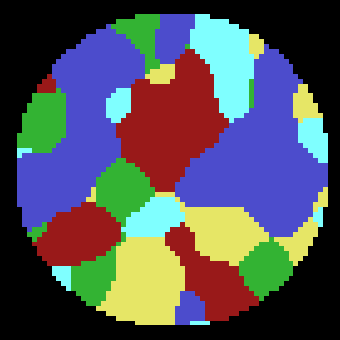
\includegraphics[width=0.12\textwidth]{figure1/kmeans_sub1} &
      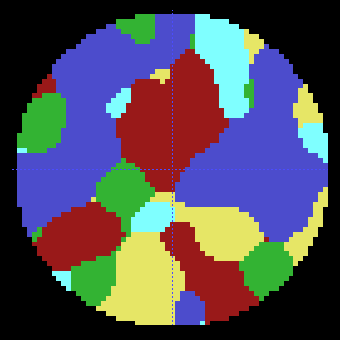
\includegraphics[width=0.12\textwidth]{figure1/ncuts_sub1} &
      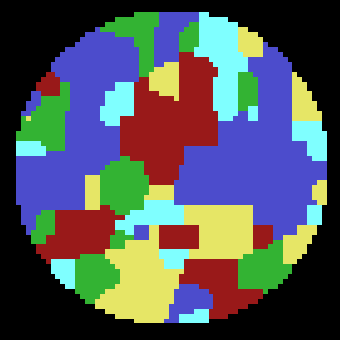
\includegraphics[width=0.12\textwidth]{figure1/mrf_sub1} \\
    \end{tabular} \\
    \hspace{15pt}
    \footnotesize
    \begin{tabular}[b]{l|ccc}
      & group & mean(sub) & var(sub) \\
      \textsf{K-means} & 92.9 & 87.0 & 0.67\\
      \textsf{N-Cuts} & 85.4 & 87.1 & 0.58 \\
      \textsf{groupmrf} & 95.7 & 97.5 & 0.59
    \end{tabular}
  \end{tabular}
\end{figure}

\end{frame}


\begin{frame}
\frametitle{Real rs-fMRI Data}

\begin{figure}[htb]
\centering
\begin{tabular}{lcc|cc|cc}
&
\multicolumn{2}{c|}{group} &
\multicolumn{2}{c|}{sub 1} &
\multicolumn{2}{c}{sub 2} \\
& $z = 26$ & $z=54$ & $z = 26$ & $z=54$ & $z = 26$ & $z=54$ \\
\begin{sideways} \footnotesize \textsf{K-Means} \end{sideways} &
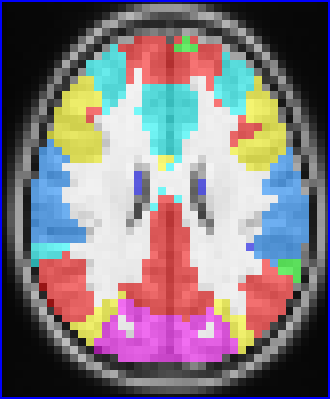
\includegraphics[width=0.13\textwidth]{figure2/kmeans_grp_z25} &
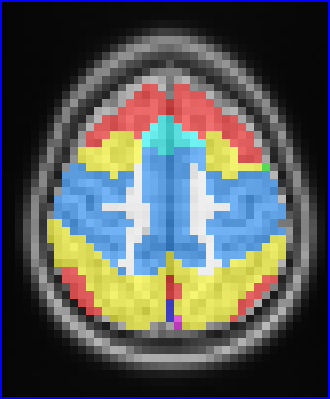
\includegraphics[width=0.13\textwidth]{figure2/kmeans_grp_z32} &
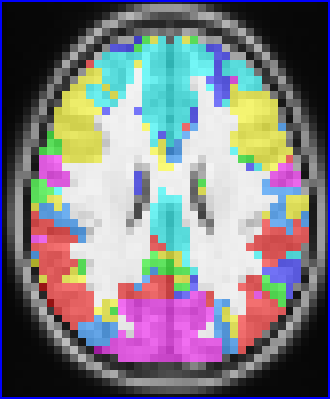
\includegraphics[width=0.13\textwidth]{figure2/kmeans_sub1_z25} &
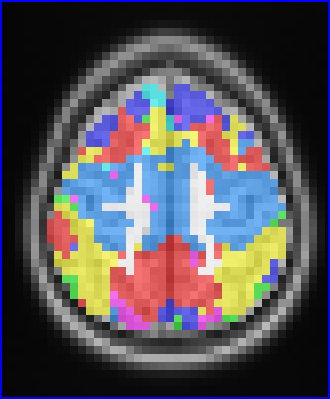
\includegraphics[width=0.13\textwidth]{figure2/kmeans_sub1_z32} &
\includegraphics[width=0.13\textwidth]{figure2/kmeans_sub2_z25} &
\includegraphics[width=0.13\textwidth]{figure2/kmeans_sub2_z32} \\
\begin{sideways} \footnotesize \textsf{N-Cuts} \end{sideways} &
\includegraphics[width=0.13\textwidth]{figure2/ncuts_grp_z25} &
\includegraphics[width=0.13\textwidth]{figure2/ncuts_grp_z32} &
\includegraphics[width=0.13\textwidth]{figure2/ncuts_sub1_z25} &
\includegraphics[width=0.13\textwidth]{figure2/ncuts_sub1_z32} &
\includegraphics[width=0.13\textwidth]{figure2/ncuts_sub2_z25} &
\includegraphics[width=0.13\textwidth]{figure2/ncuts_sub2_z32} \\
\begin{sideways} \footnotesize \textsf{groupmrf} \end{sideways} &
\includegraphics[width=0.13\textwidth]{figure2/mrf_grp_z25} &
\includegraphics[width=0.13\textwidth]{figure2/mrf_grp_z32} &
\includegraphics[width=0.13\textwidth]{figure2/mrf_sub1_z25} &
\includegraphics[width=0.13\textwidth]{figure2/mrf_sub1_z32} &
\includegraphics[width=0.13\textwidth]{figure2/mrf_sub2_z25} &
\includegraphics[width=0.13\textwidth]{figure2/mrf_sub2_z32}
\end{tabular}
\end{figure}

\end{frame}

\begin{frame}
\frametitle{Variability of Resting-State Functional Network}
\begin{block}{}
  \begin{itemize}
    \item Uncertainty: Posterior mean and variance.
    \item Variability: Spatial pattern's shape change.
  \end{itemize}
\end{block}
\end{frame}

\begin{frame}
\frametitle{Posterior mean and variance}
\begin{block}{posterior variance}
  the sample variance of the network label variables
  inferred from posterior density.
\end{block}
  Preliminary results shows the  probability of network labels
  estimated from samples drawn from posterior density.
\begin{figure}[htb]
  \centering
  \begin{tabular}[b]{cc|cc|cc}
    \multicolumn{2}{c}{sub1} &
    \multicolumn{2}{c}{sub2} &
    \multicolumn{2}{c}{sub3} \\
    \includegraphics[width=0.12\textwidth]{figure3/dmn_a} &
    \includegraphics[width=0.12\textwidth]{figure3/dmn_s} &
    \includegraphics[width=0.12\textwidth]{figure3/dmn_sub17_a} &
    \includegraphics[width=0.12\textwidth]{figure3/dmn_sub17_s} &
    \includegraphics[width=0.12\textwidth]{figure3/dmn_sub21_a} &
    \includegraphics[width=0.12\textwidth]{figure3/dmn_sub21_s} \\
    \includegraphics[width=0.12\textwidth]{figure3/atten_a} &
    \includegraphics[width=0.12\textwidth]{figure3/atten_s} &
    \includegraphics[width=0.12\textwidth]{figure3/atten_sub17_a} &
    \includegraphics[width=0.12\textwidth]{figure3/atten_sub17_s} &
    \includegraphics[width=0.12\textwidth]{figure3/atten_sub21_a} &
    \includegraphics[width=0.12\textwidth]{figure3/atten_sub21_s} 
  \end{tabular}
  \includegraphics[width=0.03\textwidth]{figure3/colorbar}
\end{figure}
\end{frame}

\begin{frame}
\frametitle{Variability: Spatial pattern's shape change}
\begin{block}{}
  \begin{itemize}
  \item The variability of Multivariate labels across can be represented by shape changes.
  \item Multivariate pattern analysis method: principal component analysis, etc.
  \end{itemize}
\end{block}
\vspace{10pt}
\includegraphics[width=0.9\textwidth]{sfig/vari}
\end{frame}

\begin{frame}
\frametitle{Timeline}
\begin{block}{}
  \begin{itemize}
  \item \textbf{Fall 2012:} Network variability analysis.
  \item \textbf{Spring 2013}: Submit a journal paper on the hierarchical
    model. Continue on variability analysis.
  \item \textbf{Summer 2013}: Dissertation writing and Ph.D thesis defense.
  \end{itemize}
\end{block}
\end{frame}

\begin{frame}
  \frametitle{Publications}

  \renewcommand{\refname}{List of Publications}
  {\footnotesize
    \begin{thebibliography}{1}

\bibitem[Liu10a]{liu2010spatialCopy}
W.~Liu, P.~Zhu, J.~Anderson, D.~Yurgelun-Todd, and P.T. Fletcher.
\newblock Spatial {R}egularization of {F}unctional {C}onnectivity {U}sing
  {H}igh-{D}imensional {M}arkov {R}andom {F}ields.
\newblock \emph{Medical Image Computing and Computer-Assisted
  Intervention--MICCAI 2010}, pages 363--370, 2010.

\bibitem[Liu11a]{liu2011monteCopy}
W.~Liu, S.~Awate, J.~Anderson, D.~Yurgelun-Todd, and P.T. Fletcher.
\newblock Monte {C}arlo {E}xpectation {M}aximization with {H}idden {M}arkov
  {M}odels to {D}etect {F}unctional {N}etworks in {R}esting-{S}tate {fMRI}.
\newblock \emph{Machine Learning in Medical Imaging}, pages 59--66, 2011.

\bibitem[Liu12a]{Liu2012aCopy}
W.~Liu, S.~Awate, and P.T. Fletcher.
\newblock Group analysis of resting-state {fMRI} by hierarchical {M}arkov
  {R}andom {F}ields.
\newblock \emph{MICCAI 2012}, In Press.

\end{thebibliography}
    }
\end{frame}

\begin{frame}
  \begin{block}{}
    Thanks very much! \\
    Questions? Comments?
  \end{block}
\end{frame}

\begin{frame}
  \frametitle{Backup: Segmentation with MRF}
  \begin{figure}
    \includegraphics[width=0.3\textwidth]{sfig/mri}
    \hspace{10pt}
    \includegraphics[width=0.3\textwidth]{sfig/seg_nosmooth}
    \hspace{10pt}
    \includegraphics[width=0.3\textwidth]{sfig/seg_smooth}
  \end{figure}
\end{frame}

\begin{frame}
  \frametitle{Neighbor System and Cliques}
  \begin{columns}[c]
    \begin{column}{6cm}
      Cliques for a 4-neighbor system.
      \end{column}

    \begin{column}{5cm}
      \includegraphics[width=0.9\textwidth]{sfig/clique_1}
    \end{column}
    \end{columns}
\end{frame}


\begin{frame}
  \frametitle{Bayesian Inference: Gibbs Sampling At Voxel Level}
  \begin{block}{}
    \begin{align*}
&p(x_s | x_{-s},Y) \propto \frac{1}{Z_s}\exp\{-U(x_s | x_{-s})\} \cdot p(y_s | x_s) \\
&= \frac{1}{Z_s}\exp\{-U_p(x_s | x_{\cN_s }, y_s)\} \nonumber\\
& U_p = \alpha\!\sum_{j=1}^J \psi(x_s, x_{\tilde s}^j) + \beta\!\!\sum_{r\in \cN_{s}} \psi(x_s,x_r), \quad \forall s \in \cV_G,\\
& U_p = \alpha \psi(x_s,x_{\tilde s}) + \beta\!\!\sum_{r\in \cN_{s}} \psi (x_s, x_r) - \kappa_l \mu_l\T y_s - \log C_p, \: \forall s \in \cV_H^j.
\end{align*}
    \end{block}
  \includegraphics[width=0.6\textwidth]{sfig/voxelgibbs}

\end{frame}

\end{document}
